\documentclass[spanish,aspectratio=169]{beamer}
\usepackage[spanish]{babel}
\usepackage[T1]{fontenc}
\usepackage[utf8]{inputenc}

\usepackage{mathpazo}
\usepackage[euler-digits,euler-hat-accent]{eulervm}
\usepackage{subcaption}
\usepackage{amsmath,amssymb}
\usepackage[separate-uncertainty=true,multi-part-units=single]{siunitx}
\usepackage{pgf}
\usepackage{fix-cm}

\usetheme[sectionpage=none]{metropolis}

\title [Desarrollo de un instrumento para la detección de neutrones solares]{Desarrollo de un instrumento para la detección de neutrones solares en la cima del Volcán Sierra Negra}
\author{\texorpdfstring{Marcos Anzorena Méndez\newline\url{anzorena@geofisica.unam.mx}}{Marcos Anzorena Méndez}}
\date{8 de Septiembre de 2021}
\institute{Instituto de Geofísica\\
Universidad Nacional Autónoma de México}

\begin{document}

\maketitle


\section
[El Origen de los rayos cósmicos]{El Origen de los rayos cósmicos}
\frame{\sectionpage}


\begin{frame}{Origen de los rayos cósmicos}

\begin{figure}
	\centering
	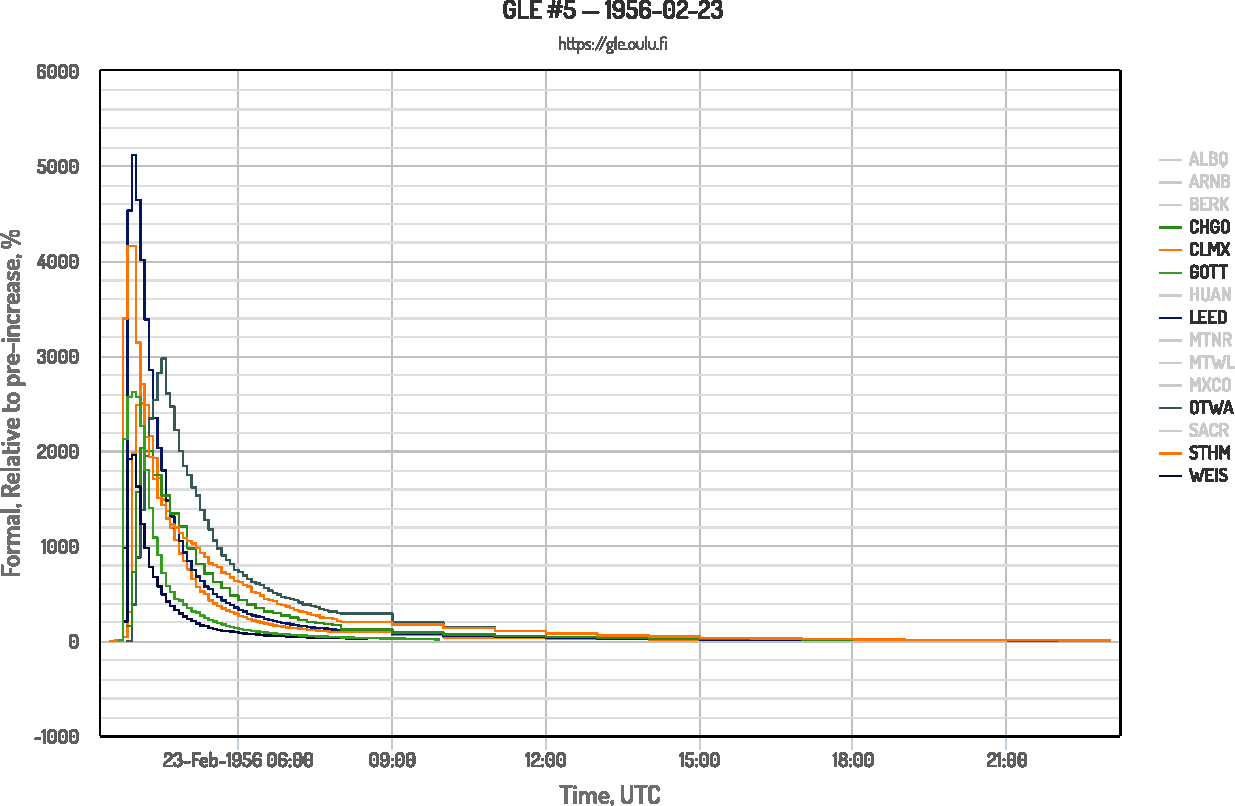
\includegraphics[width=0.8\textwidth]{GLE.oulu.fi.pdf}
\end{figure}

\end{frame}

\begin{frame}{Origen de los rayos cósmicos}

\begin{figure}
	\centering
	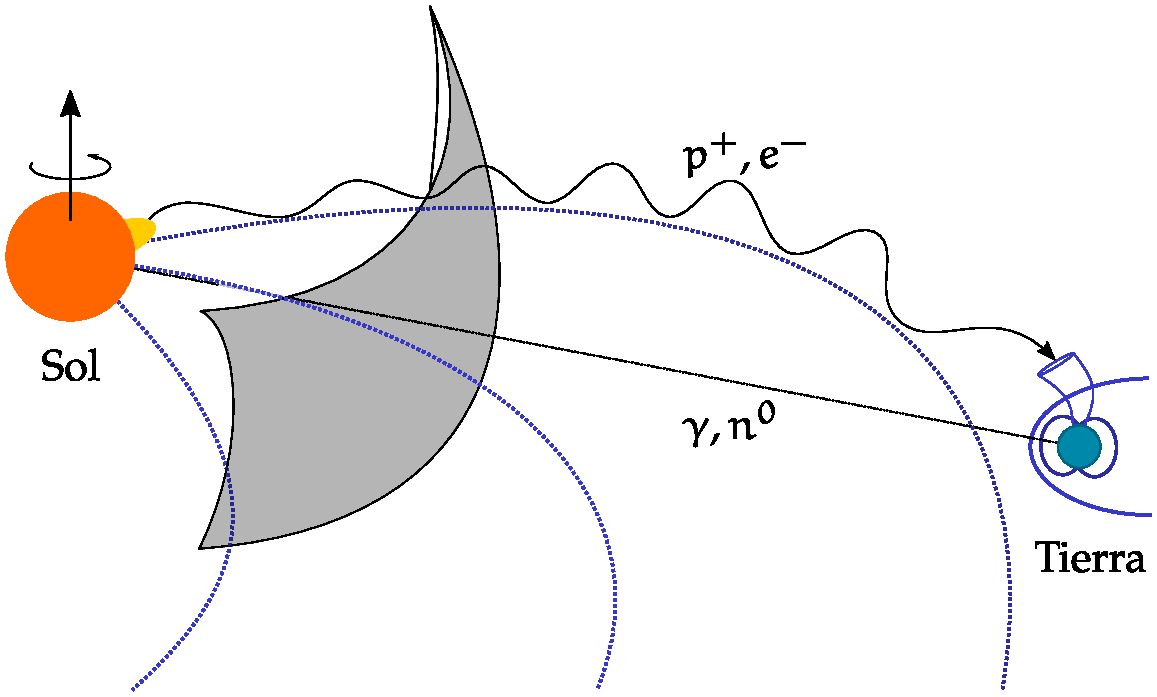
\includegraphics[width=0.9\textwidth]{solar-neutron.pdf}
\end{figure}

\end{frame}

\begin{frame}{Detección en superficie}

\begin{figure}
	\centering
	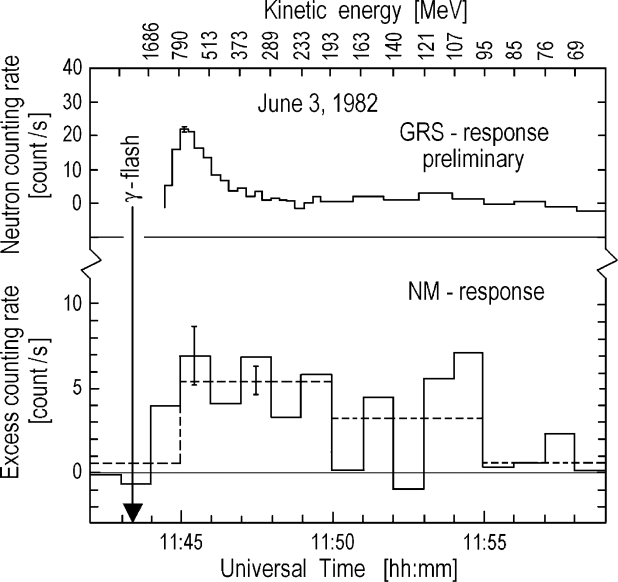
\includegraphics[width=0.55\textwidth]{neutrons-ground.png}
\end{figure}

\end{frame}

\begin{frame}{Detección en superficie}

\begin{figure}
	\centering
	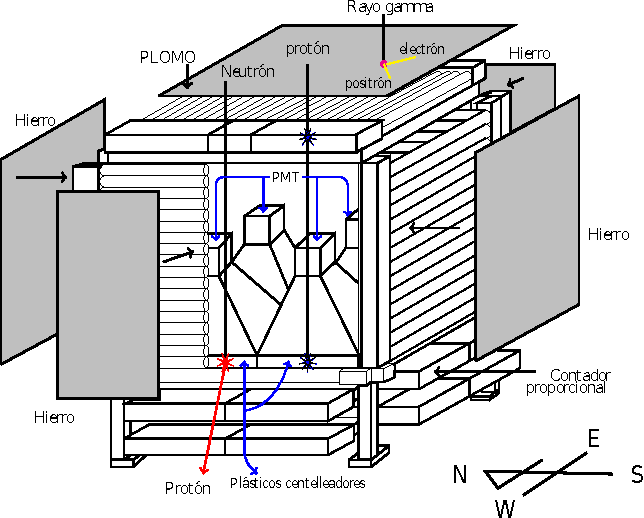
\includegraphics[width=0.6\textwidth]{tns-mexico.pdf}
\end{figure}

\end{frame}

\begin{frame}{Telescopio centellador de rayos cósmicos (SciCRT)}

\begin{figure}
        \centering
        \begin{subfigure}[b]{0.45\textwidth}
                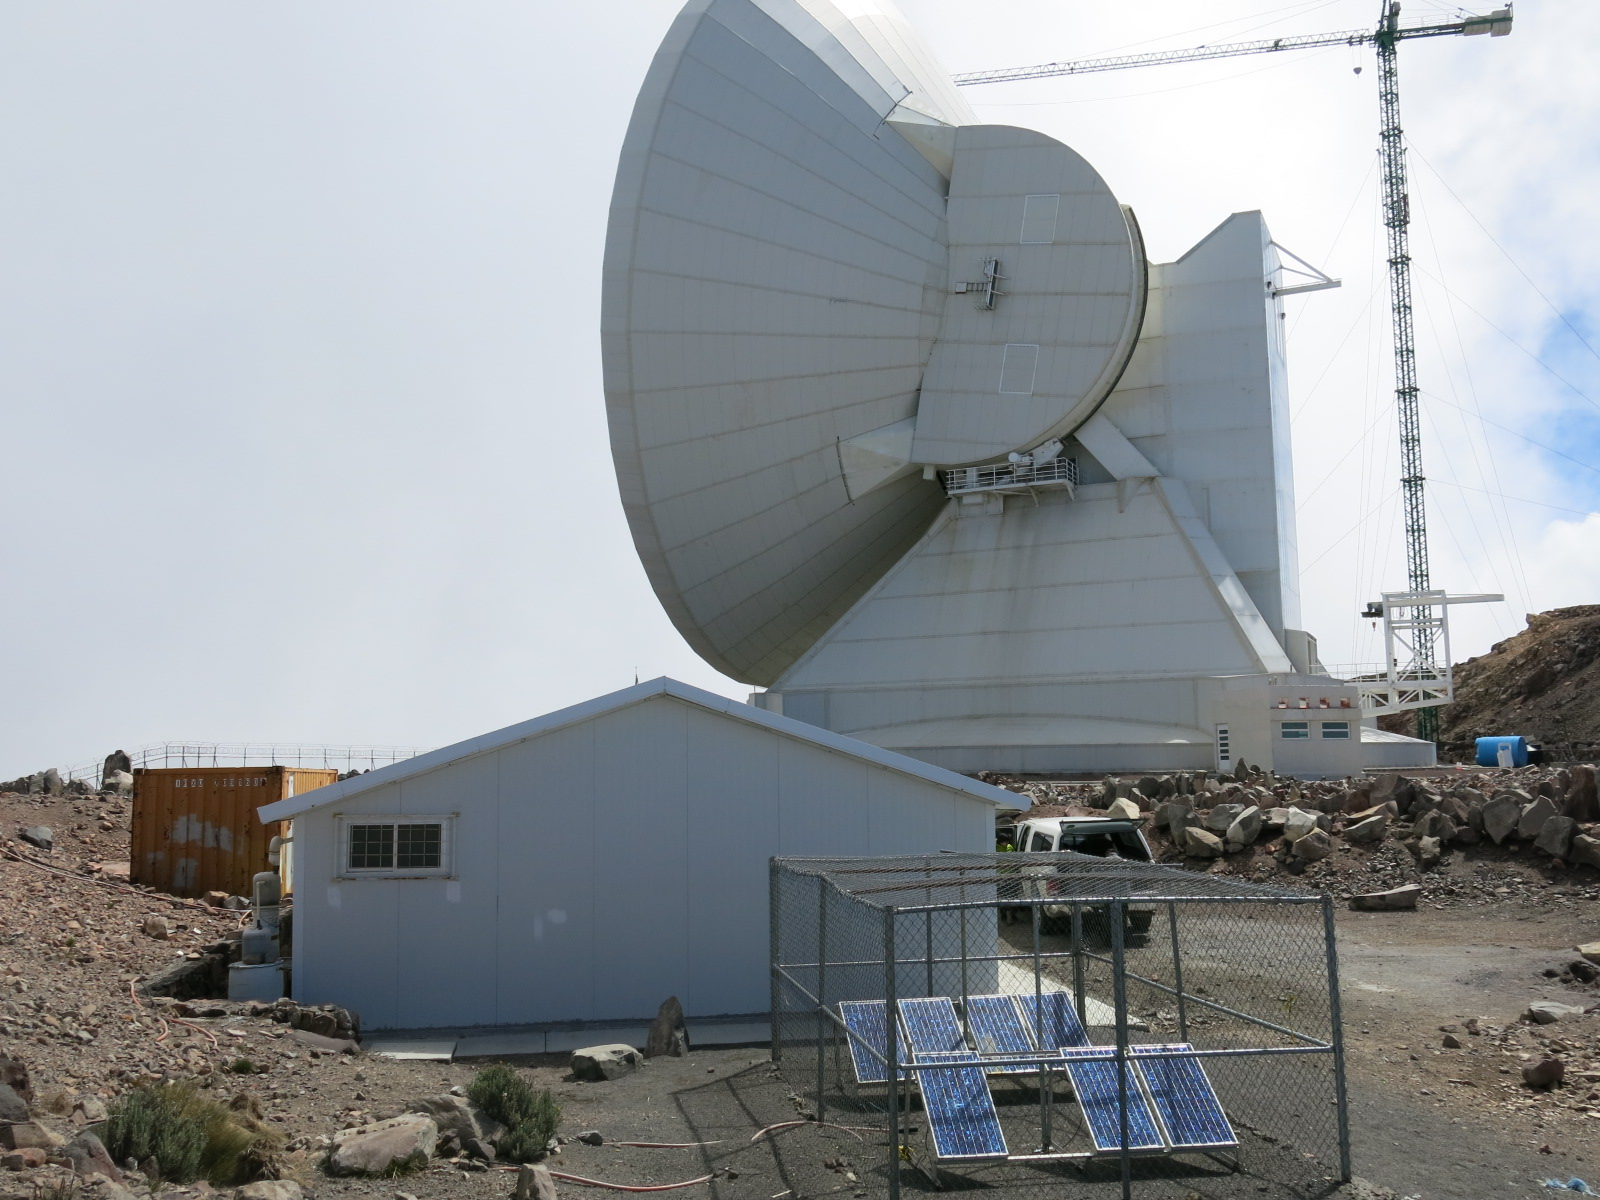
\includegraphics[width=6.0cm]{sn-scicrt.jpg}
        \end{subfigure}
        \begin{subfigure}[b]{0.45\textwidth}
                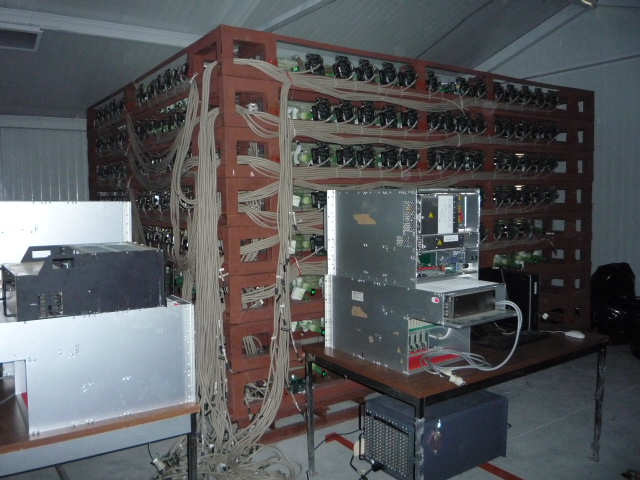
\includegraphics[width=6.0cm]{scicrt-full.jpg}
        \end{subfigure}
\end{figure}
\end{frame}


\section
[Desarrollo de la nueva electrónica y validación experimental]{Desarrollo de la nueva electrónica y validación experimental}
\frame{\sectionpage}


\begin{frame}{Motivación para desarrollar la nueva electrónica}

\begin{figure}
	\centering
	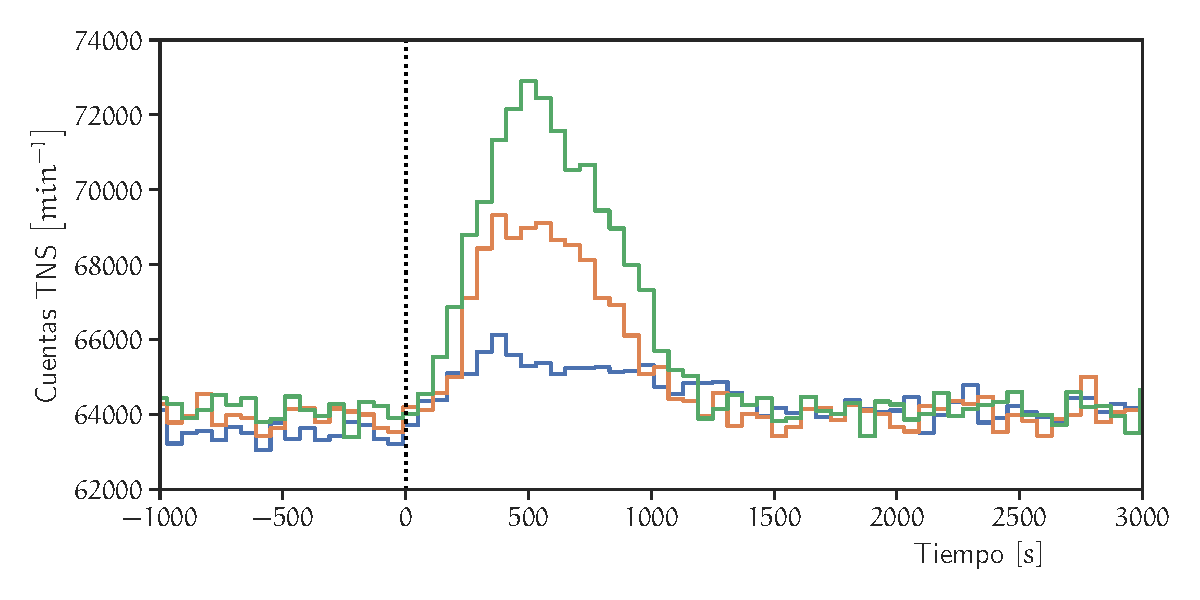
\includegraphics[width=\textwidth]{scicrt-sim.pdf}
\end{figure}

\end{frame}

\begin{frame}{Operación básica del sistema de detección}

\begin{figure}
	\centering
	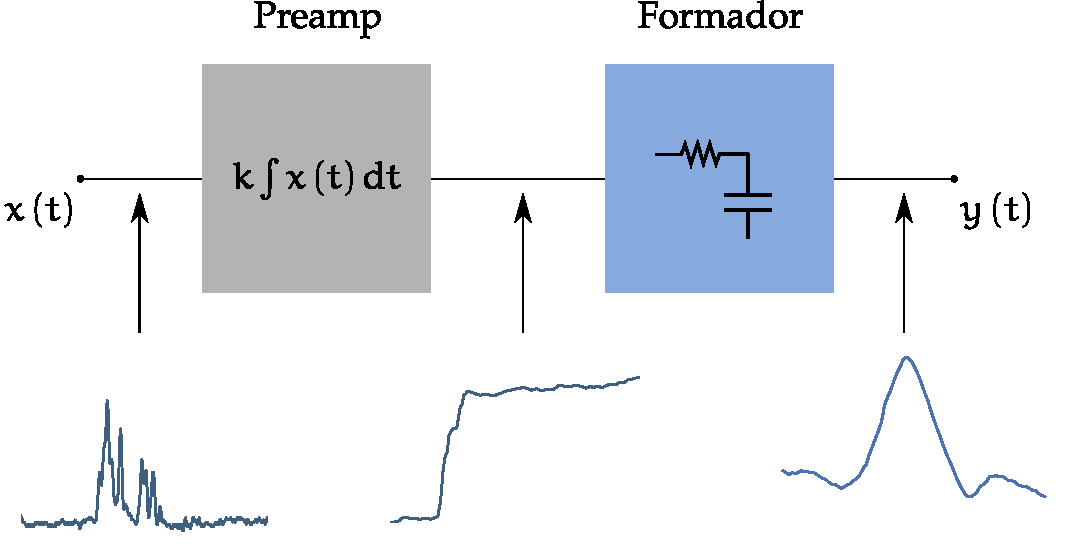
\includegraphics[width=\textwidth]{preamp-4.pdf}
\end{figure}

\end{frame}

\begin{frame}{Arquitectura propuesta}

\begin{figure}
	\centering
	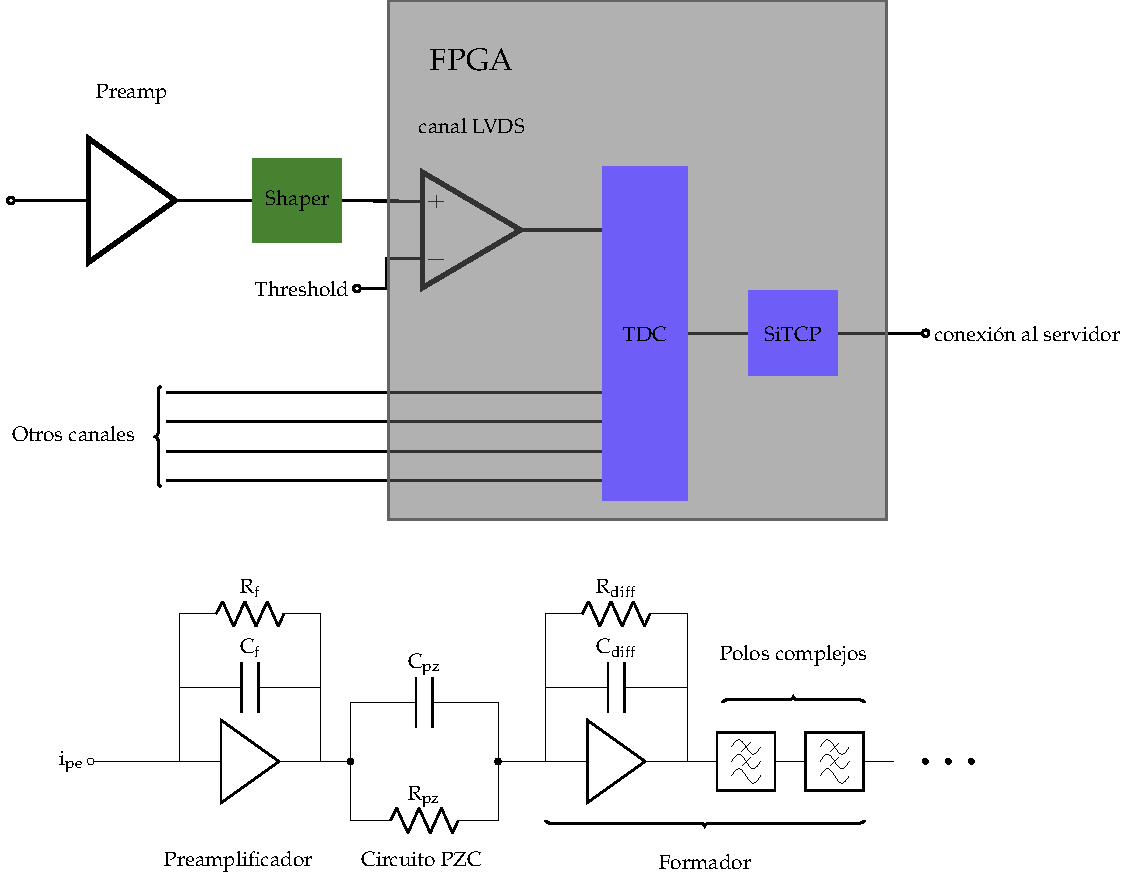
\includegraphics[width=0.7\textwidth]{nfeb-prot.pdf}
\end{figure}

\end{frame}

\begin{frame}{La técnica de time over threshold}

\begin{figure}
        \centering
        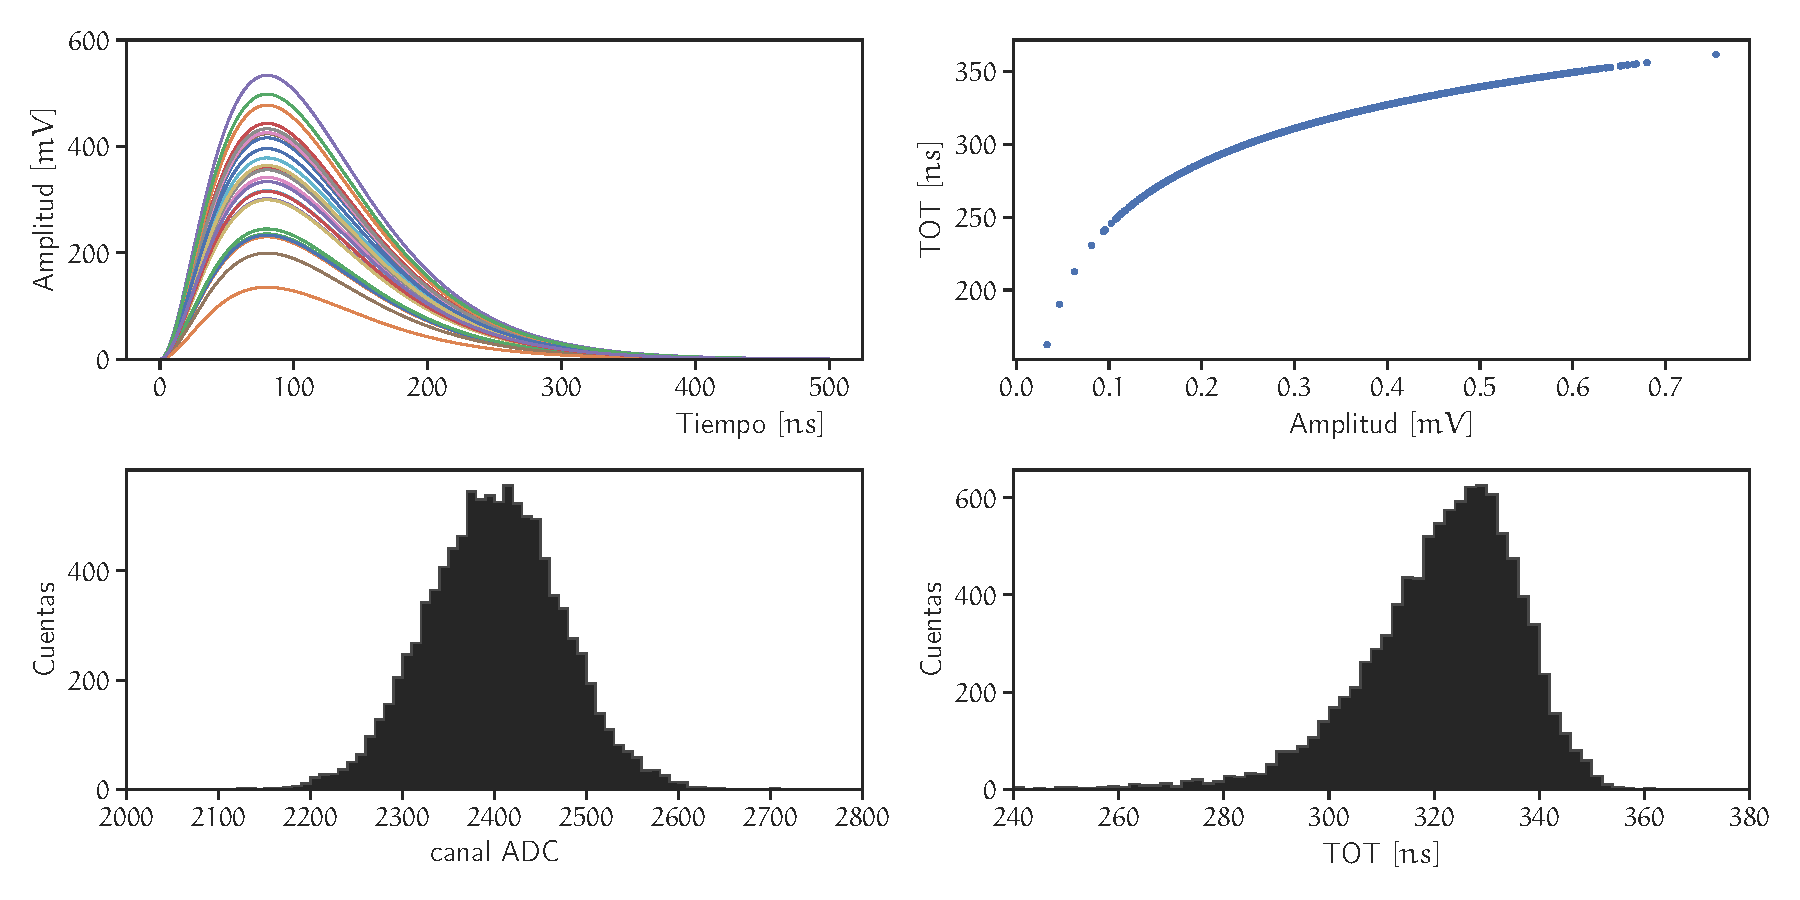
\includegraphics[width=\textwidth]{TOT-model.pdf}
\end{figure}

\end{frame}

\begin{frame}{La técnica de time over threshold}

\begin{figure}
        \centering
        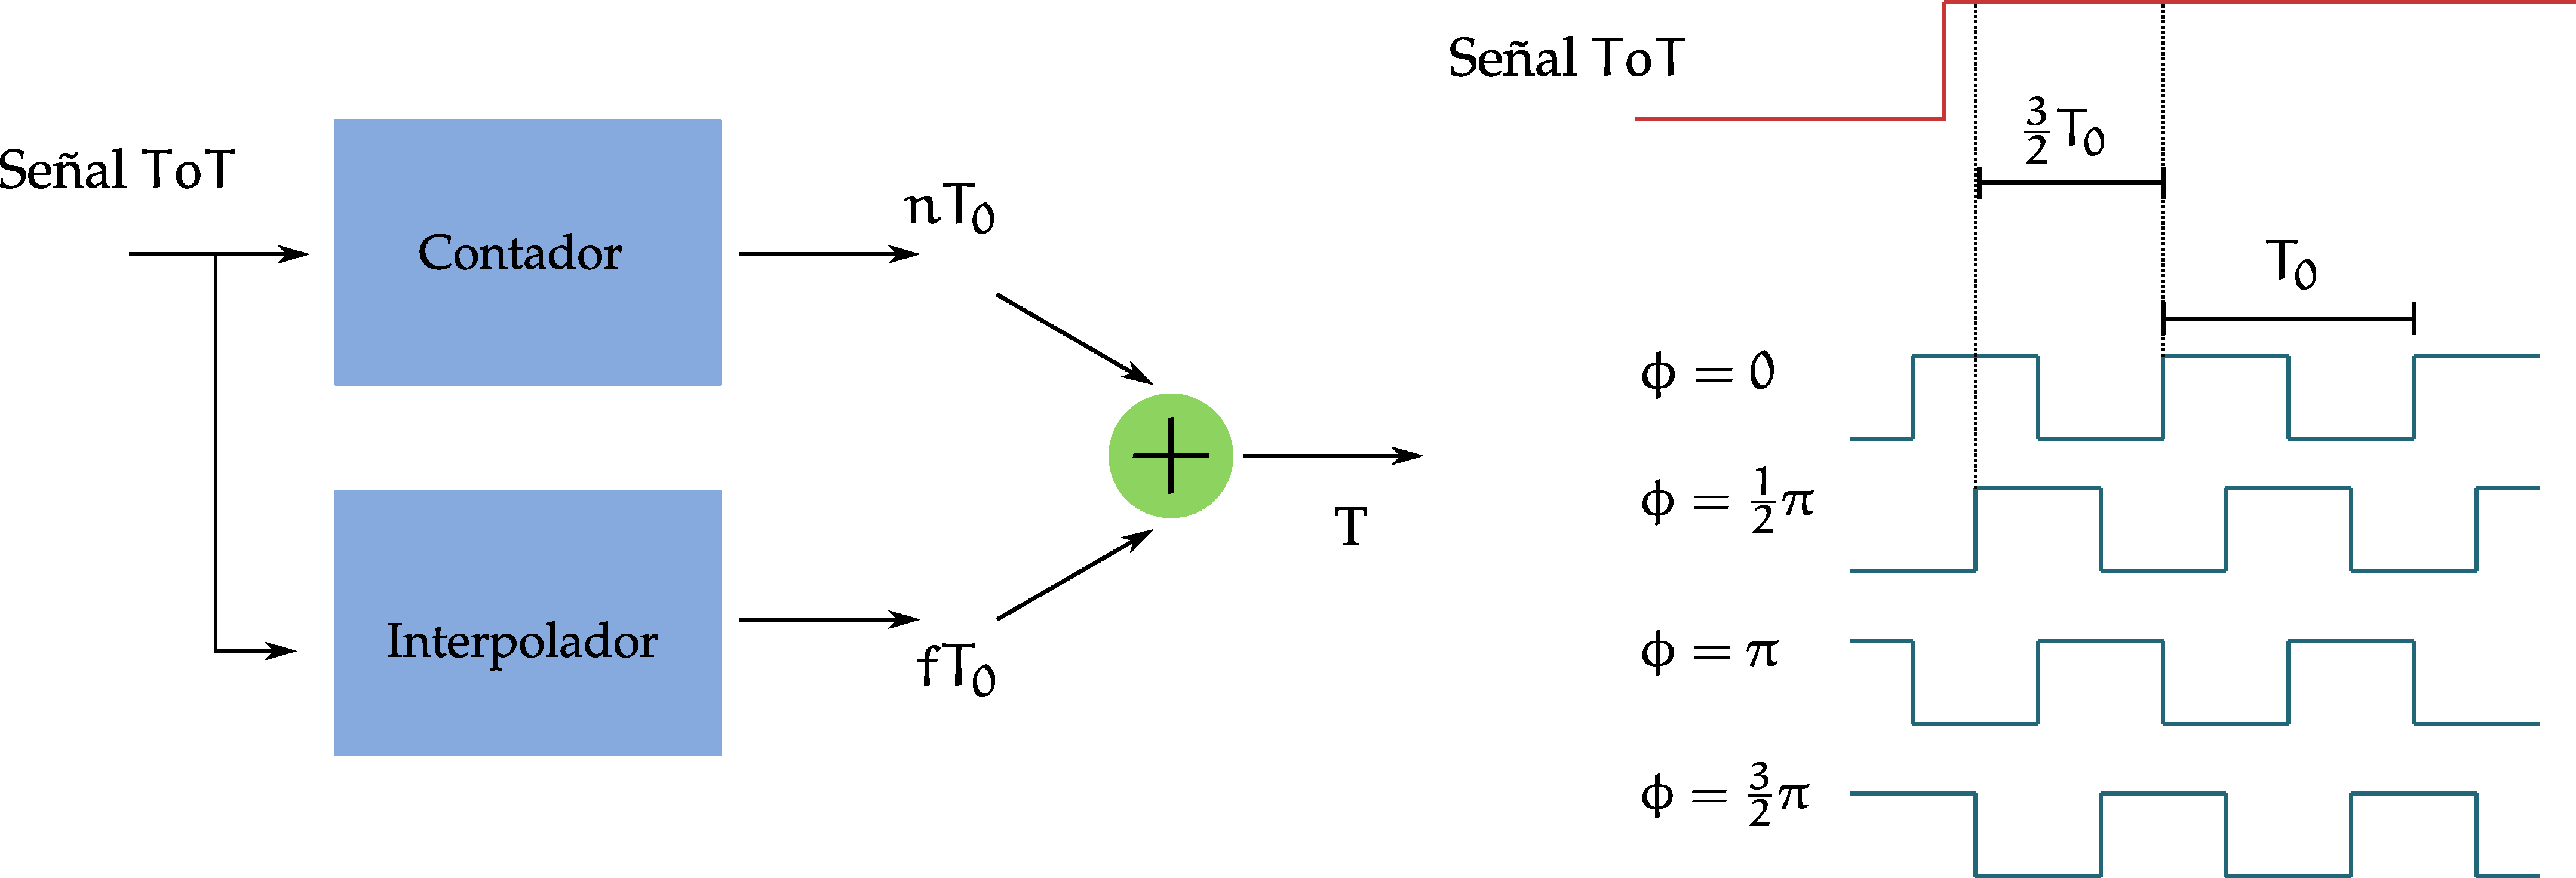
\includegraphics[width=\textwidth]{tdc-diagram.pdf}
\end{figure}

\end{frame}

\section{Diseño de la nueva electrónica mediante simulación MC}


\begin{frame}{Diseño de la nueva electrónica del Telescopio}

\begin{block}{Parámetros de diseño}

\begin{itemize}
	\item Tiempo de integración del pre-amplificador $\tau_{int}$.
	\item Ganancia total del amplificador-formador $G_{V}$.
	\item Tiempo de formación $t_{peak}$.
	\item Resolución del TDC y rango dinámico $T_{min}$, $N$ (número de bits del TDC).
	\item Máxima tasa de detección.
\end{itemize}

\end{block}

\begin{block}{Restricciones}

\begin{itemize}
	\item Consumo de potencia.
	\item Tamaño de la tarjeta
	\item Costo
	\item Rango dinámico.

\end{itemize}

\end{block}

\end{frame}

\begin{frame}{Simulación MC de una barra de centelleo}

\begin{figure}
        \centering
        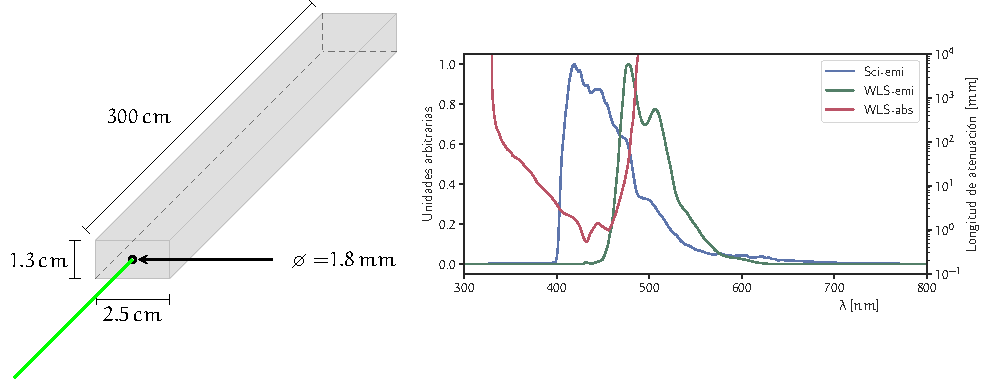
\includegraphics[width=\textwidth]{scibar.pdf}
\end{figure}

\end{frame}

\begin{frame}{Simulación MC de una barra de centelleo}

\begin{figure}
        \centering
        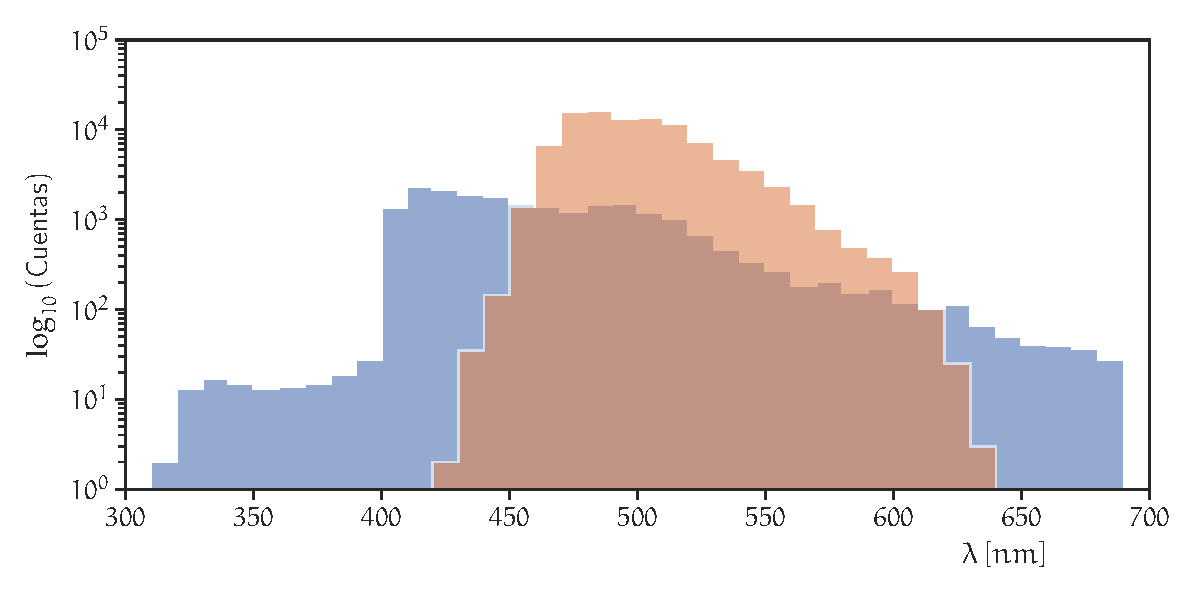
\includegraphics[width=\textwidth]{sim-optics-spect.pdf}
\end{figure}

\end{frame}

\begin{frame}{Atenuación en la fibra: experimento vs simulación}

\begin{figure}
        \centering
        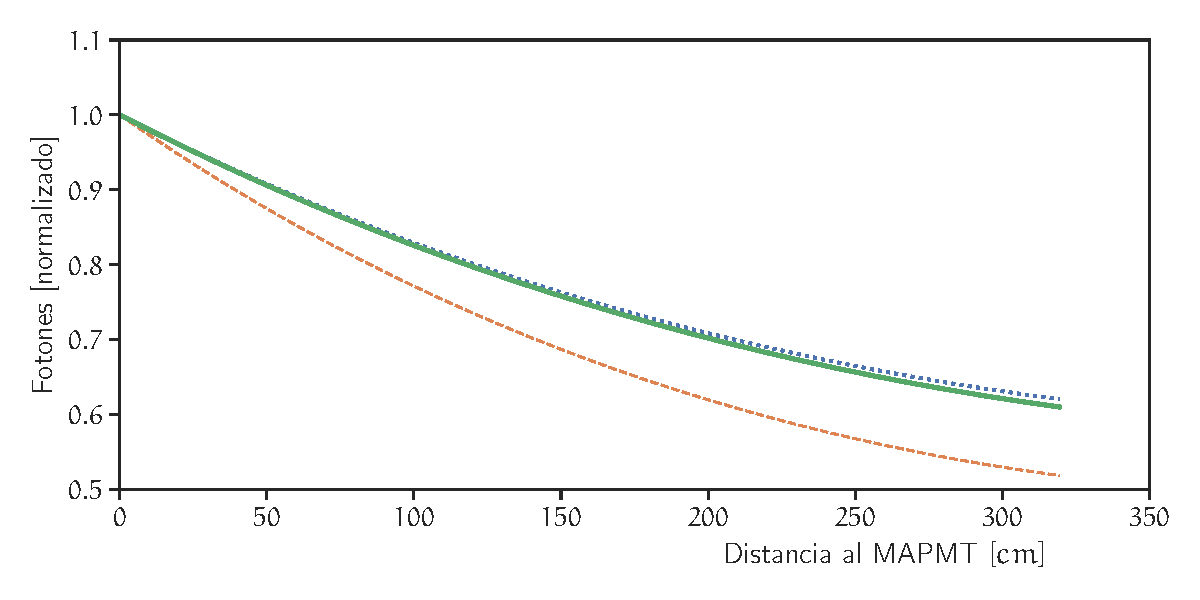
\includegraphics[width=\textwidth]{data_atlength.pdf}
\end{figure}

\end{frame}


\begin{frame}{Single photo-electron response}

\begin{figure}
        \centering
        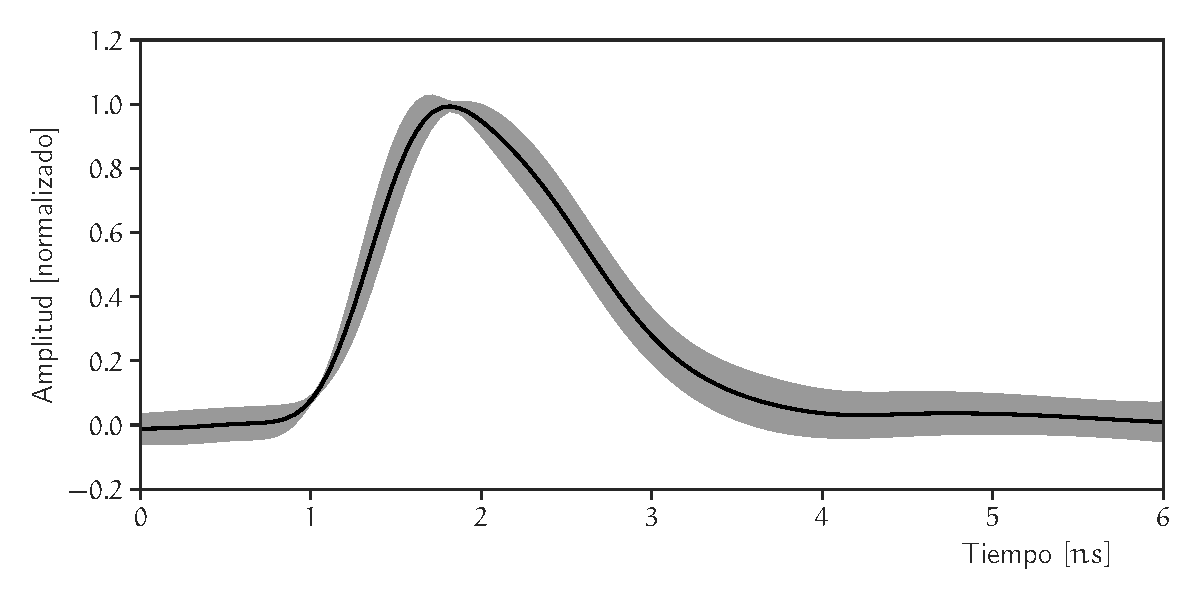
\includegraphics[width=\textwidth]{sphe-signal.pdf}
\end{figure}

\end{frame}

\begin{frame}{Prueba del prototipo}

\begin{figure}
        \centering
        \begin{subfigure}[b]{0.475\textwidth}
                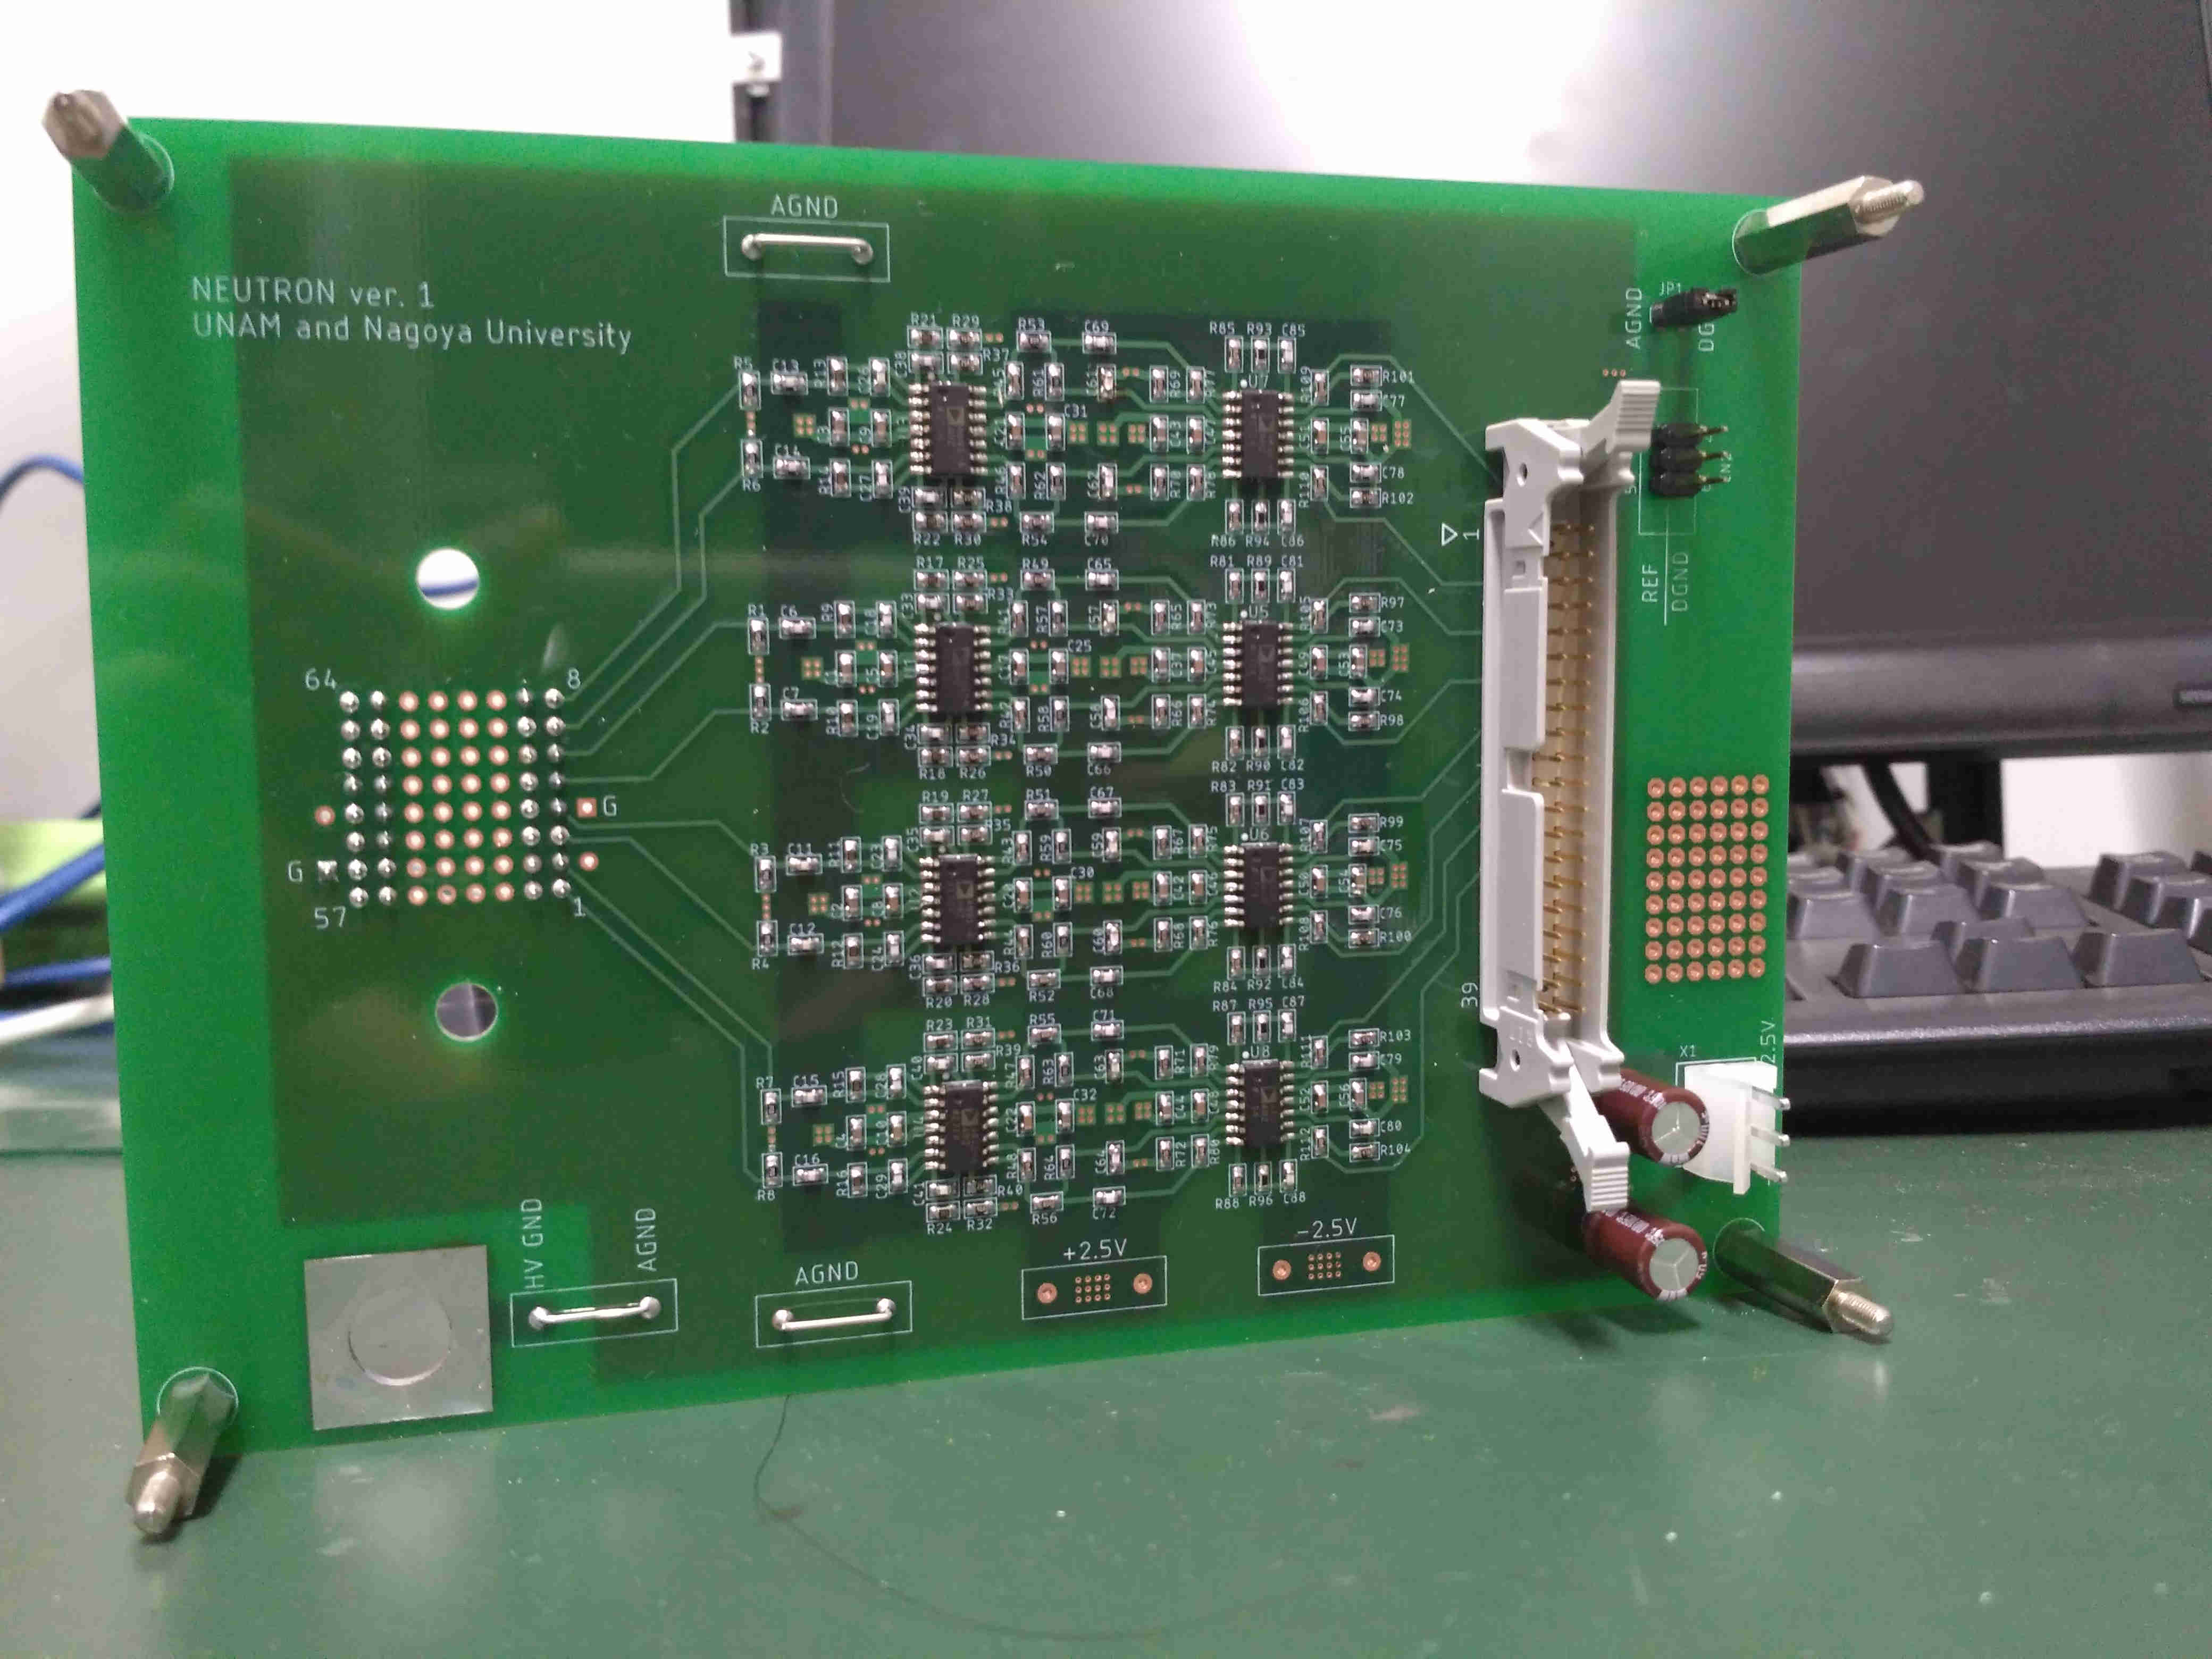
\includegraphics[width=6.5cm]{neutron_ver1.jpg}
        \end{subfigure}
        \begin{subfigure}[b]{0.475\textwidth}
                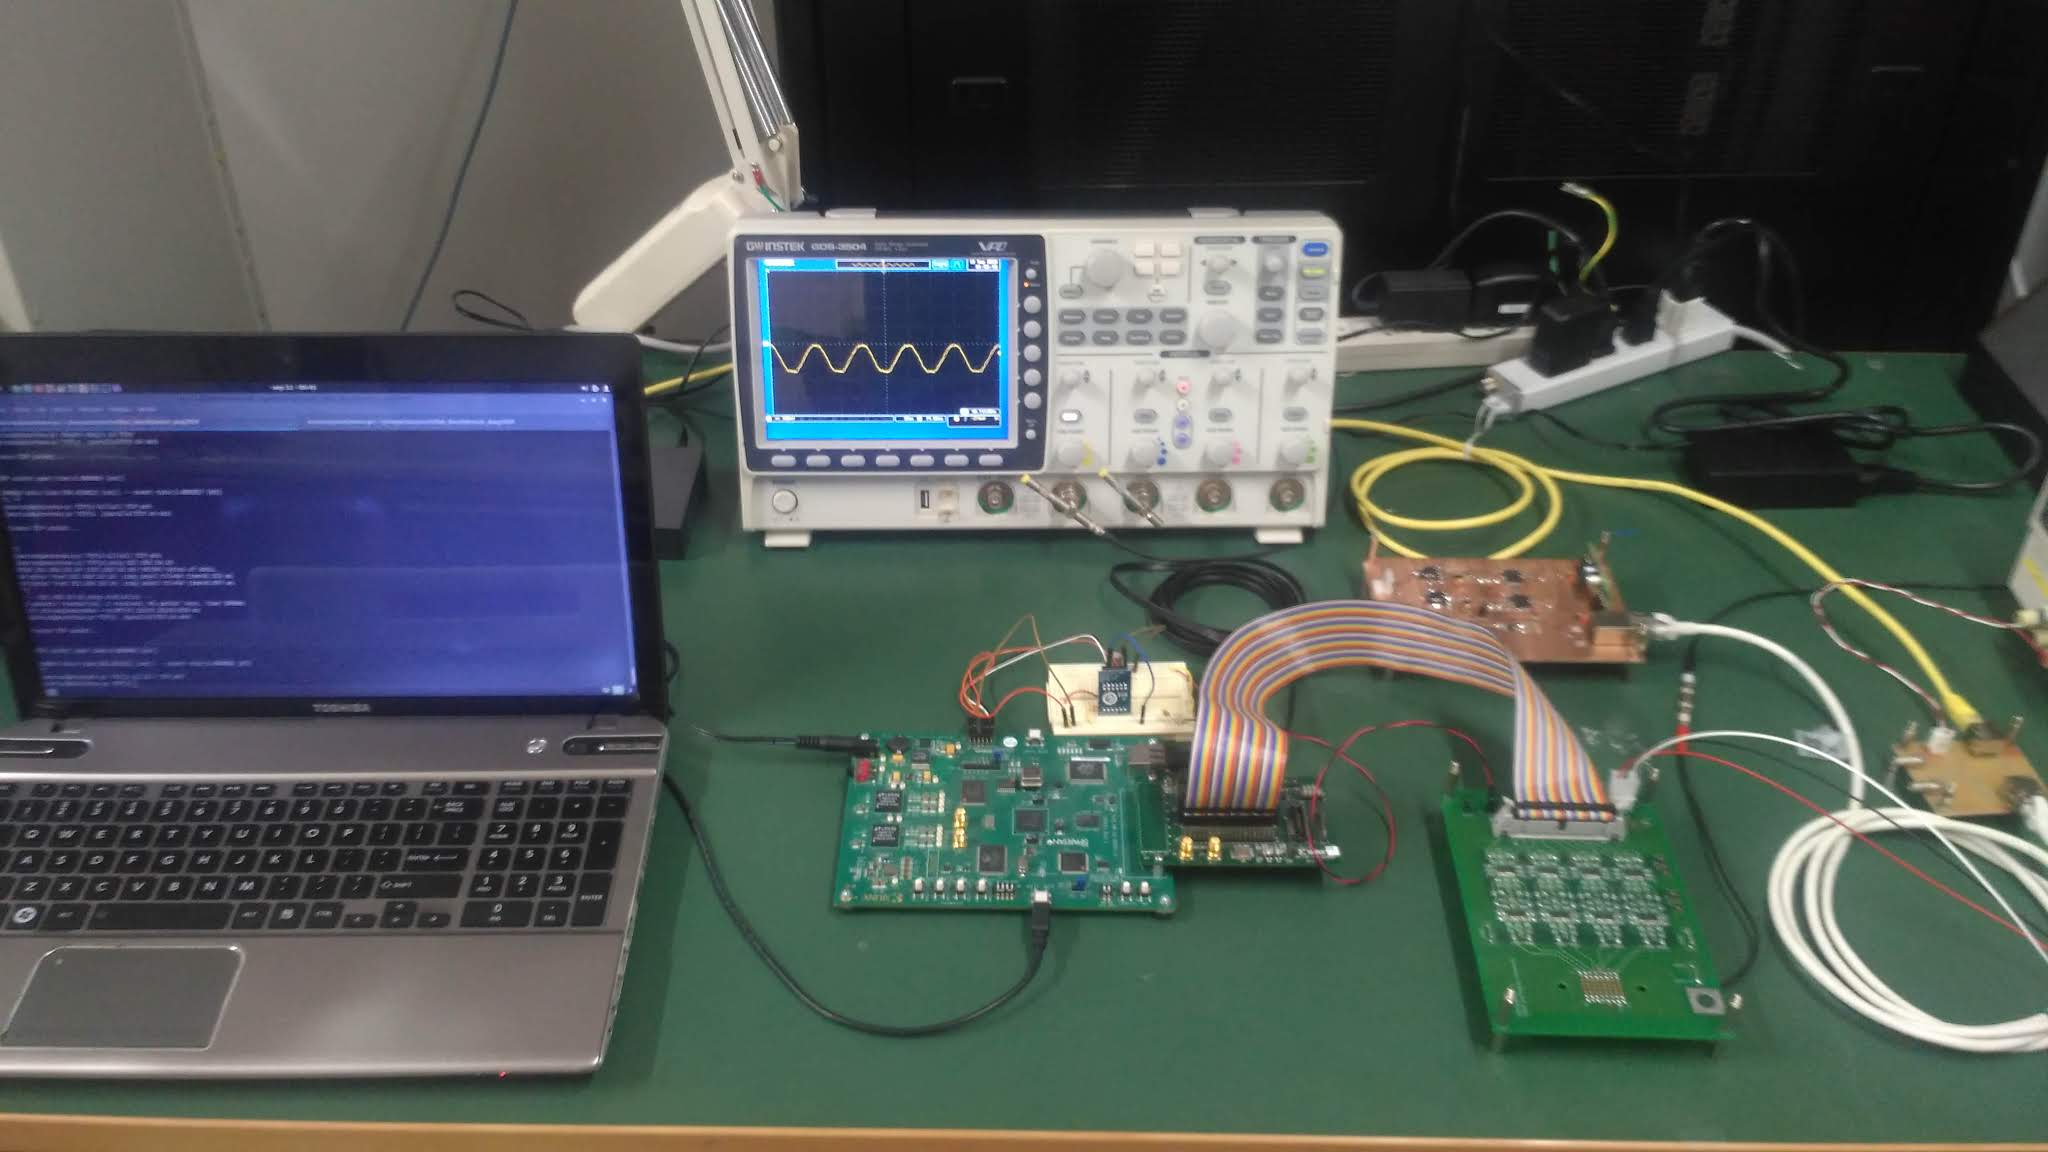
\includegraphics[width=6.5cm]{complete-system.jpg}
        \end{subfigure}
\end{figure}

\end{frame}

\begin{frame}{Prueba del prototipo}

\begin{figure}
        \centering
        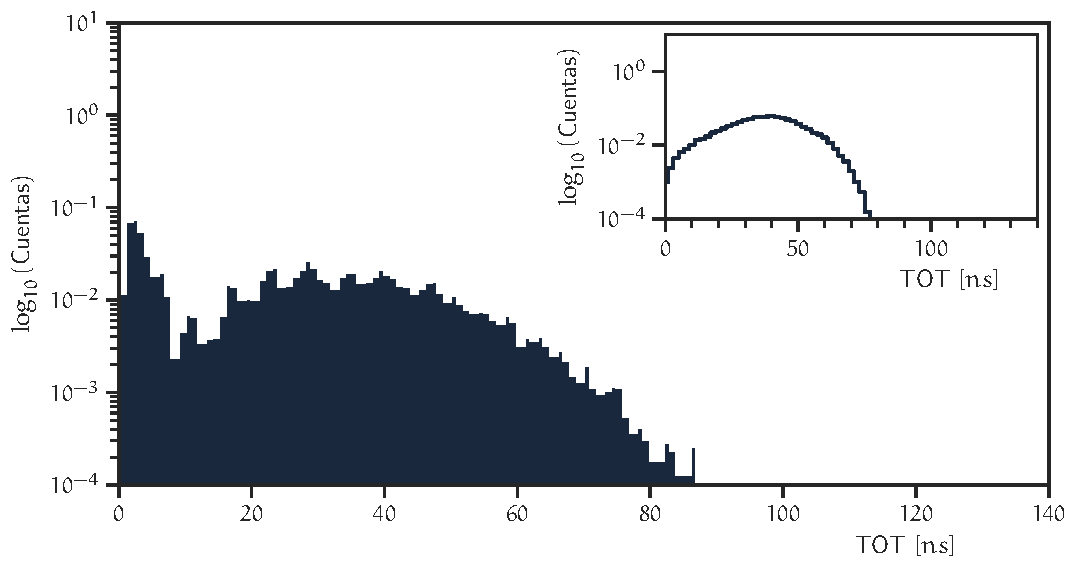
\includegraphics[width=\textwidth]{tdc_sim-exp.pdf}
\end{figure}

\end{frame}


\begin{frame}{Validación experimental de la simulación en SN}

\begin{figure}
          \centering
          \begin{subfigure}[b]{0.45\textwidth}
                  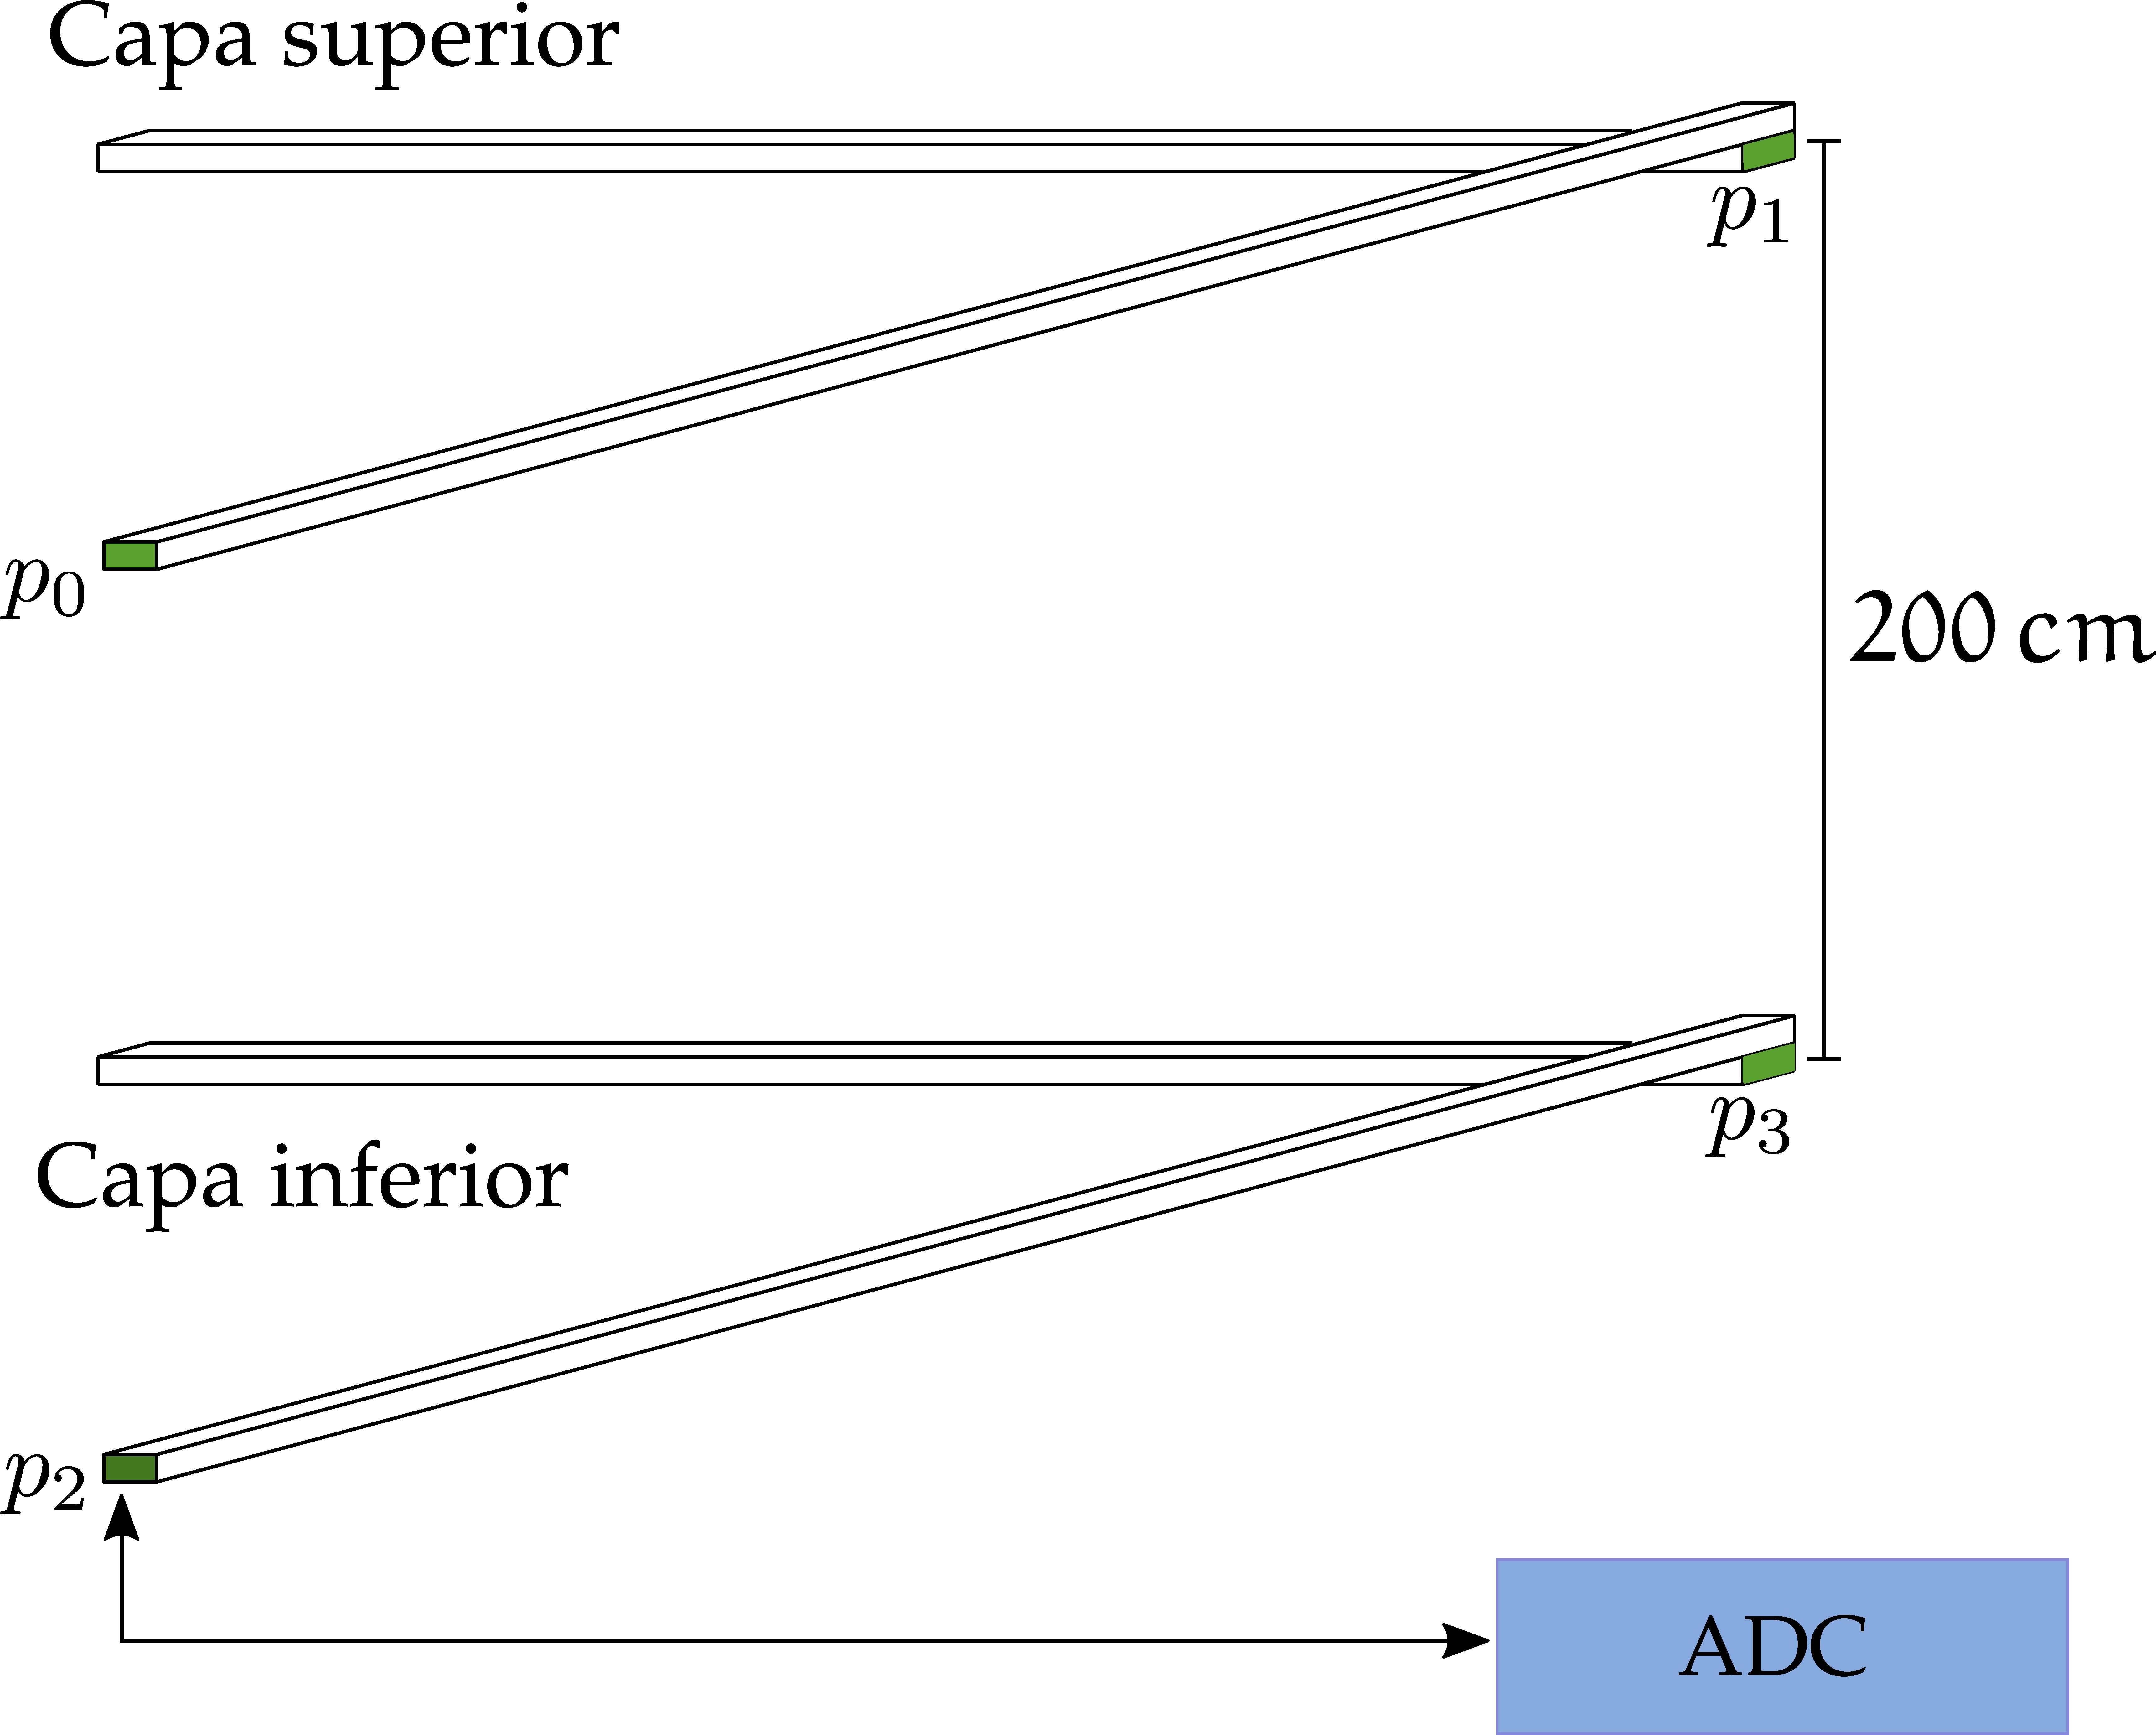
\includegraphics[width=6.3cm]{muons-experiment-0.pdf}
          \end{subfigure}
          \begin{subfigure}[b]{0.45\textwidth}
                  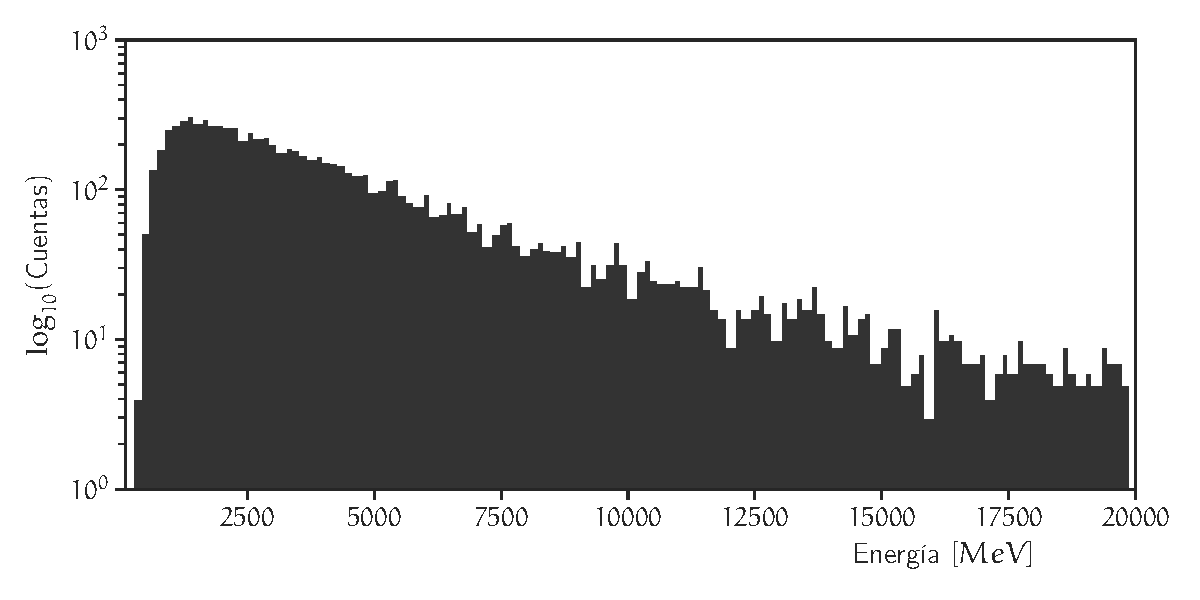
\includegraphics[width=6.3cm]{scibar-edep.pdf}
          \end{subfigure}
\end{figure}

\end{frame}

\begin{frame}{Validación experimental de la simulación en SN}

\begin{figure}
        \centering
        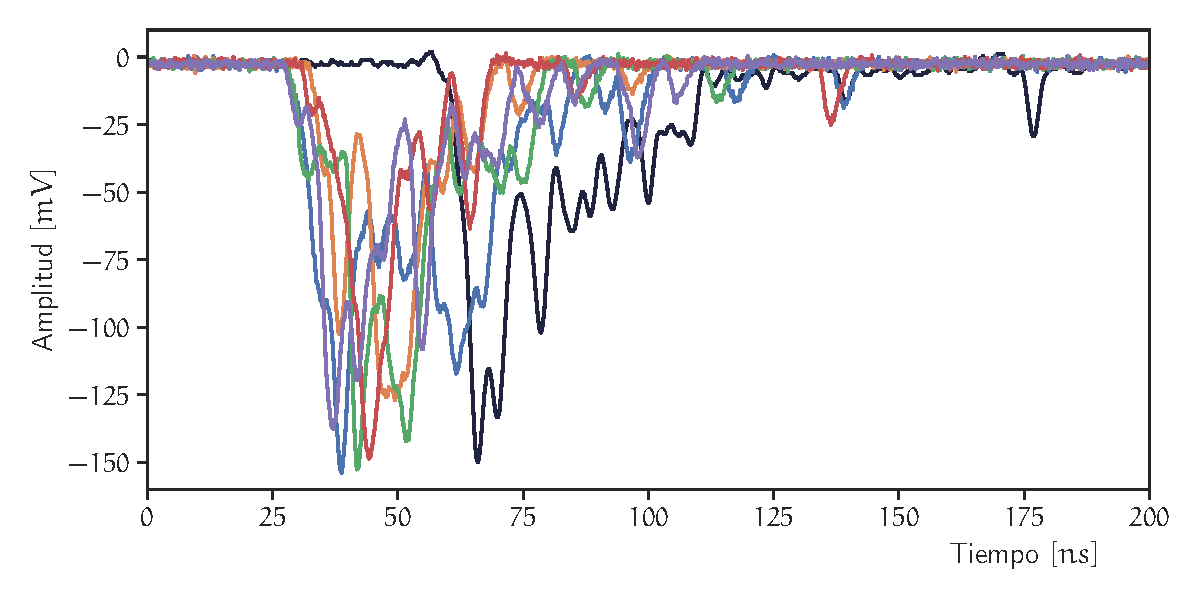
\includegraphics[width=\textwidth]{muon-pulse.pdf}
\end{figure}

\end{frame}

\begin{frame}{Validación experimental de la simulación en SN}

\begin{figure}
        \centering
        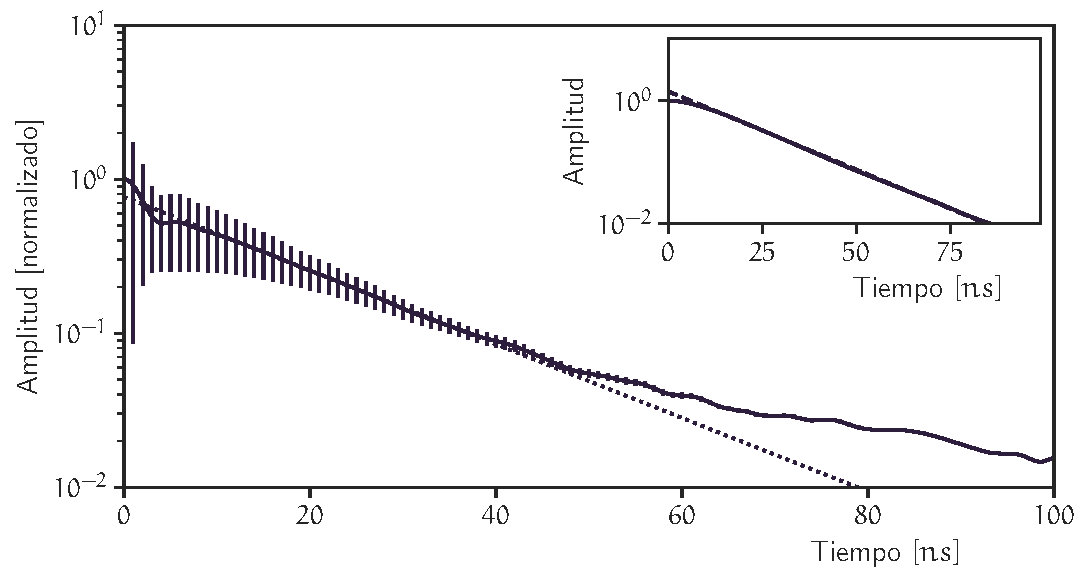
\includegraphics[width=\textwidth]{muons-tail-fit.pdf}
\end{figure}

\end{frame}

\begin{frame}{Validación experimental de la simulación en SN}

\begin{figure}
        \centering
        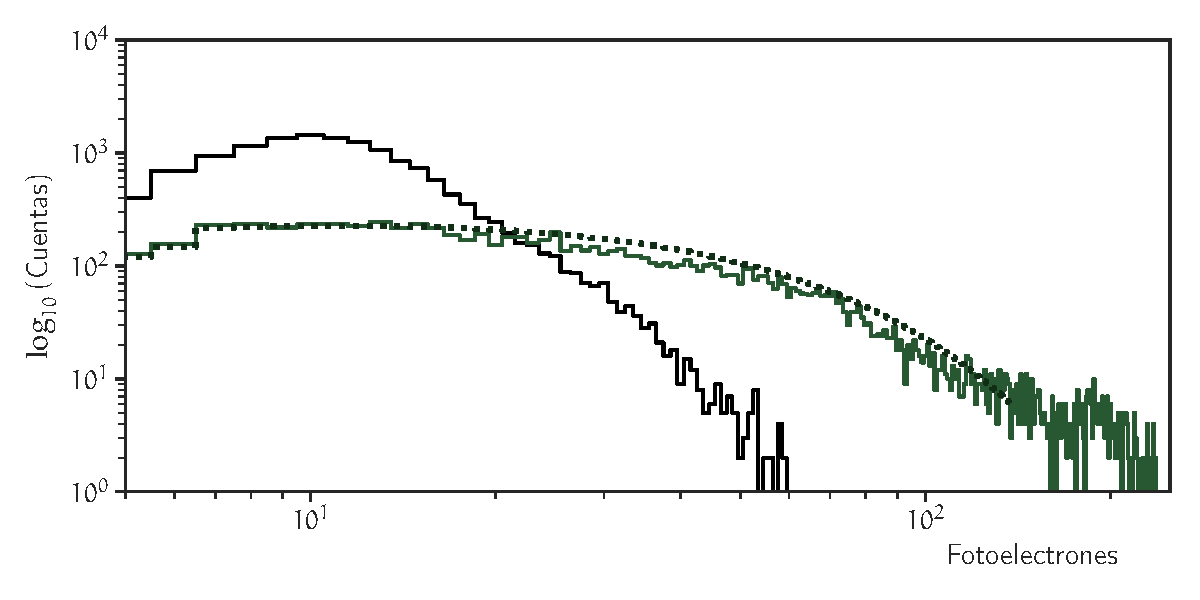
\includegraphics[width=\textwidth]{photons-number.pdf}
\end{figure}

\end{frame}

\section
[Desempeño del SciCRT y análisis de eventos]{Desempeño del SciCRT y análisis de eventos}
\frame{\sectionpage}

\begin{frame}{Evaluación del desempeño}

\begin{minipage}{0.45\textwidth}
  \begin{itemize}
      \item Partículas inyectadas en la simulación: neutrones, protones, $\mu^{\pm}$, $e^{\pm}$ y rayos $\gamma$.
      \item Utilizar el modelo PARMA como generador de eventos.
      \item Rango de las partículas: \SI{10}{\mega\electronvolt} a \SI{1}{\tera\electronvolt}.
      \item Los propiedades ópticas del detector están deshabilitadas.
  \end{itemize}
\end{minipage}
\begin{minipage}{0.45\textwidth}
  \begin{figure}
    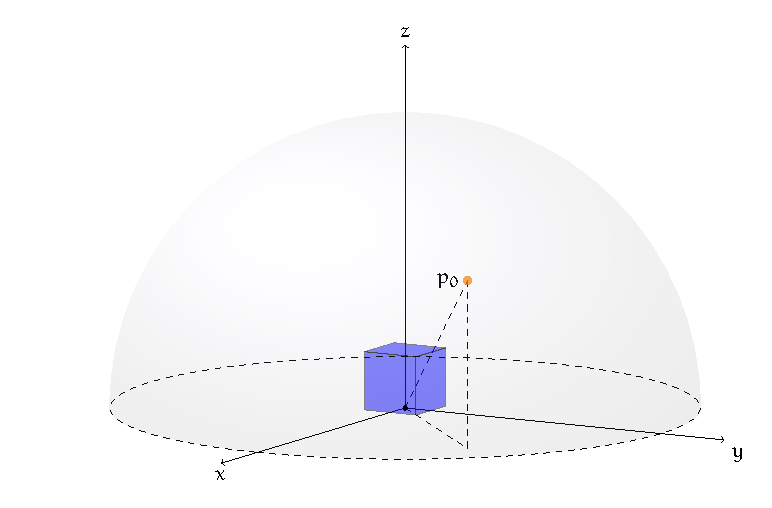
\includegraphics[width=6.3cm]{sim-setup.pdf}
  \end{figure}
\end{minipage}

\end{frame}

\begin{frame}{Evaluación del desempeño}

\begin{figure}
        \centering
        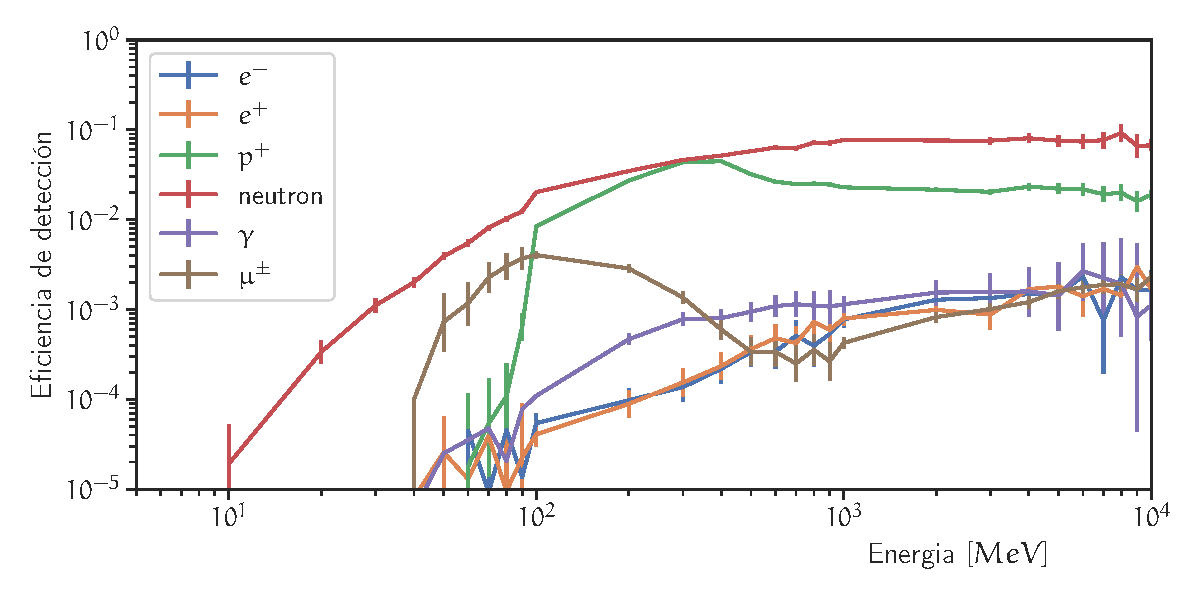
\includegraphics[width=0.9\textwidth]{scibar-efficiency.pdf}
\end{figure}

\textcolor{red}{Tasa de eventos: \SI{3132.31(9480)}{eventos \per\minute}}

\end{frame}

\begin{frame}{Evaluación del desempeño}

\begin{figure}
        \centering
        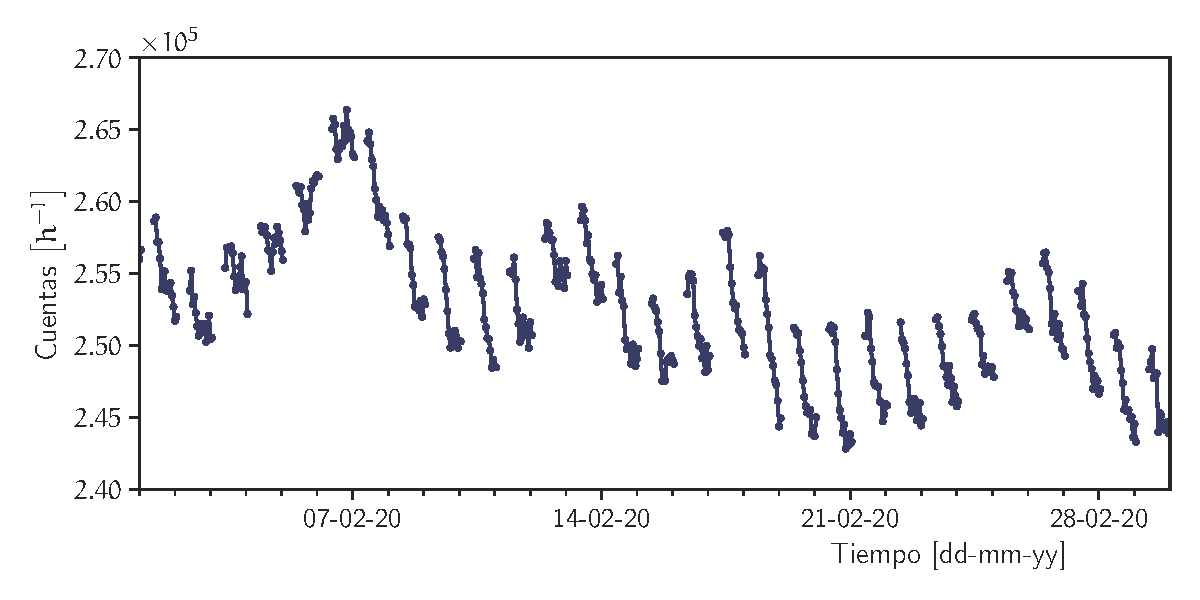
\includegraphics[width=0.9\textwidth]{neutron-monthly.pdf}
\end{figure}

\textcolor{red}{Tasa de eventos: \SI{3178.40(177)}{eventos \per\minute}}

\end{frame}

\begin{frame}{Estabilidad del detector}

\begin{figure}
        \centering
        \begin{subfigure}[b]{0.49\textwidth}
                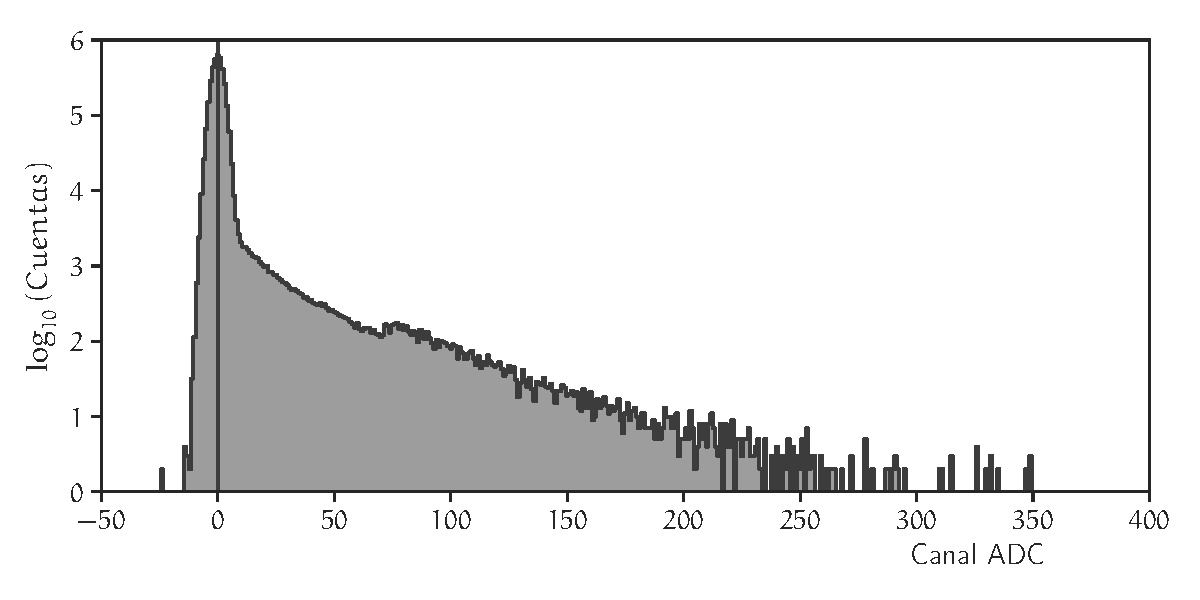
\includegraphics[width=6.85cm]{neutron-ped.pdf}
        \end{subfigure}
        \begin{subfigure}[b]{0.49\textwidth}
                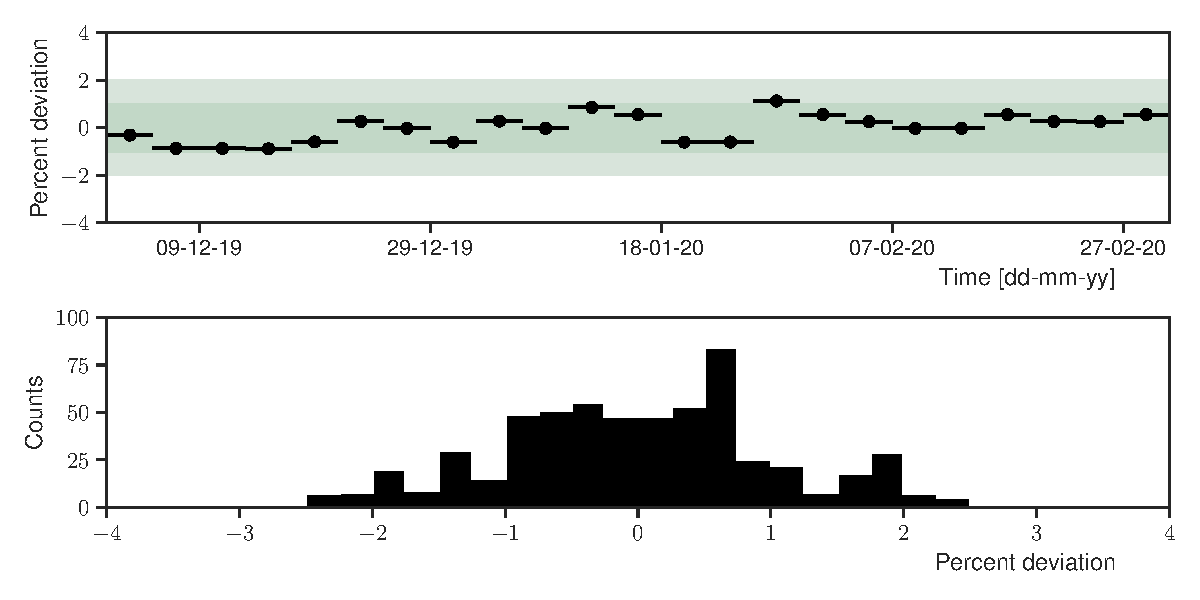
\includegraphics[width=6.85cm]{neutron-mip_stability.pdf}
        \end{subfigure}
\end{figure}

\end{frame}

\begin{frame}{Posible observación de neutrones el 04/09/17}

\begin{figure}
        \begin{subfigure}[b]{0.49\textwidth}
                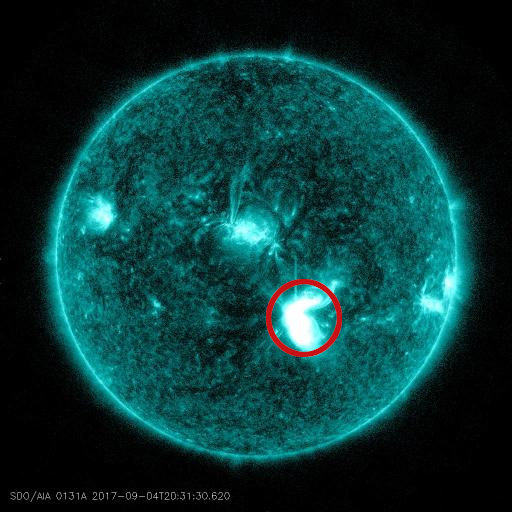
\includegraphics[width=6.85cm]{sdo170904-2030-13.jpg}
        \end{subfigure}
        \begin{subfigure}[b]{0.49\textwidth}
                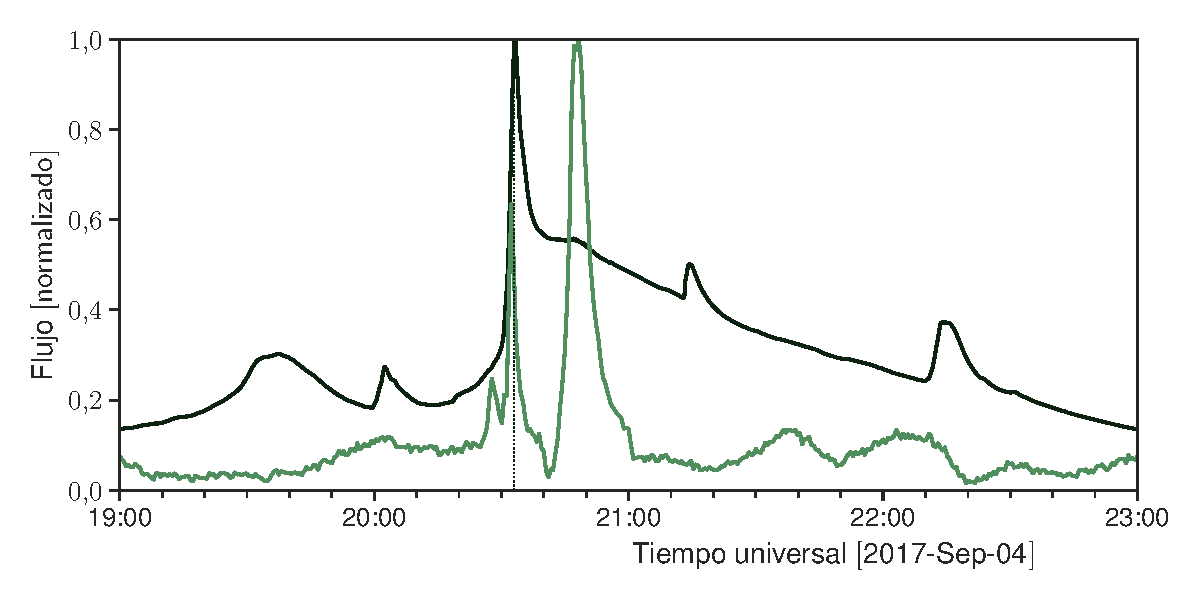
\includegraphics[width=6.85cm]{xrays_170904.pdf}
        \end{subfigure}
\end{figure}

\end{frame}


\begin{frame}{Clasificación de eventos}

\begin{figure}
        \centering
        \begin{subfigure}[b]{0.49\textwidth}
                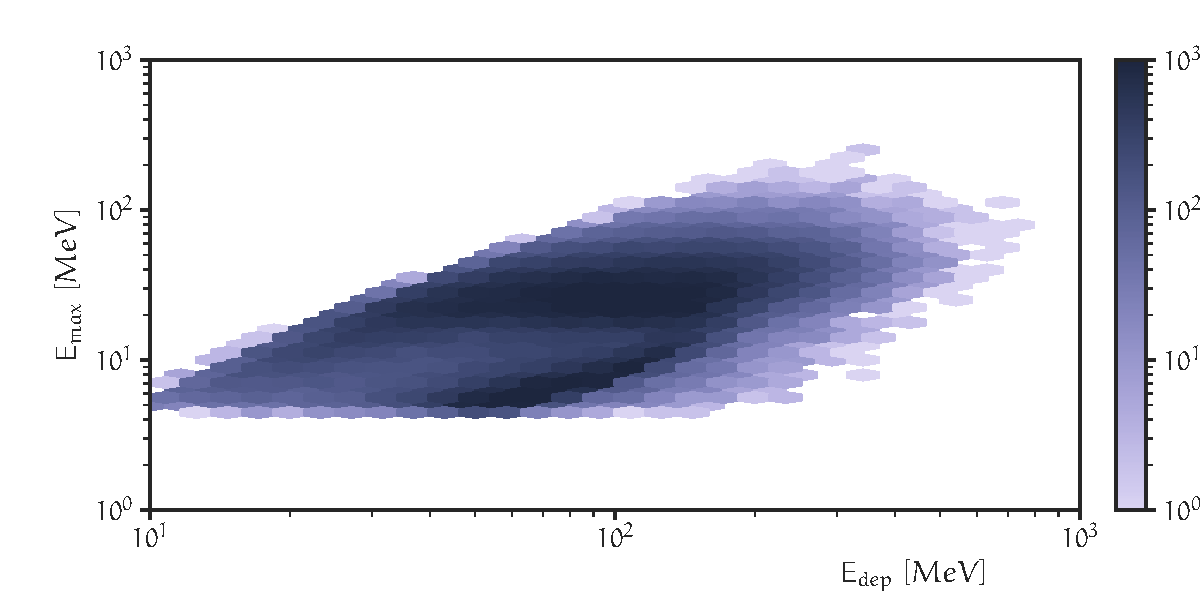
\includegraphics[width=6.85cm]{scibar-had.pdf}
        \end{subfigure}
        \begin{subfigure}[b]{0.49\textwidth}
                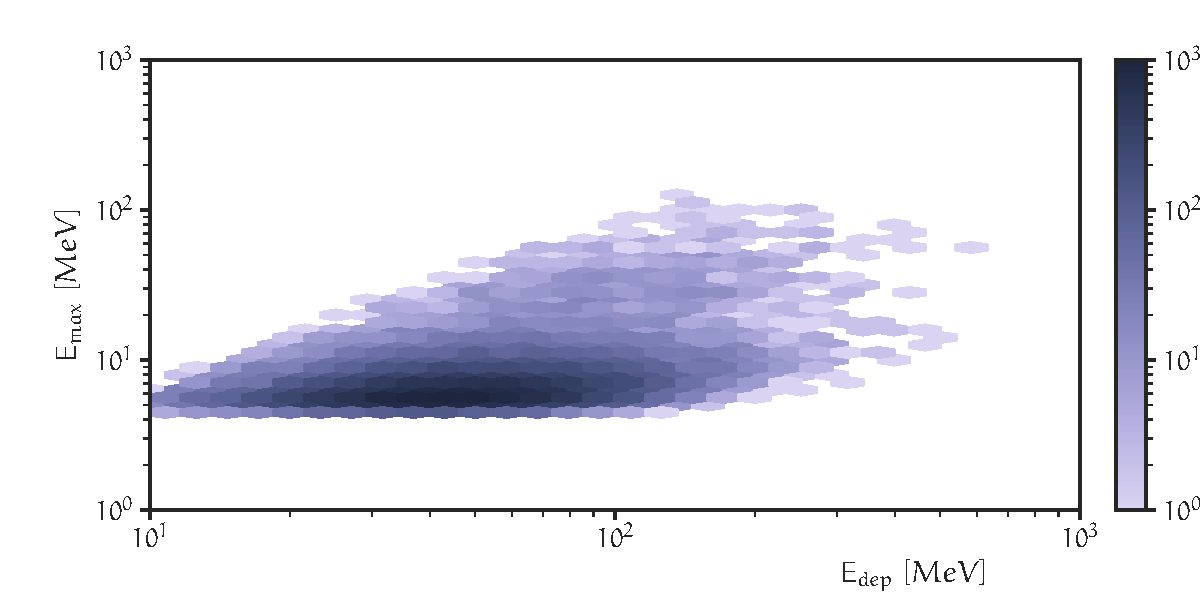
\includegraphics[width=6.85cm]{scibar-em.pdf}
        \end{subfigure}
\end{figure}

\end{frame}

\begin{frame}{Resultados del análisis}

\begin{figure}
        \centering
        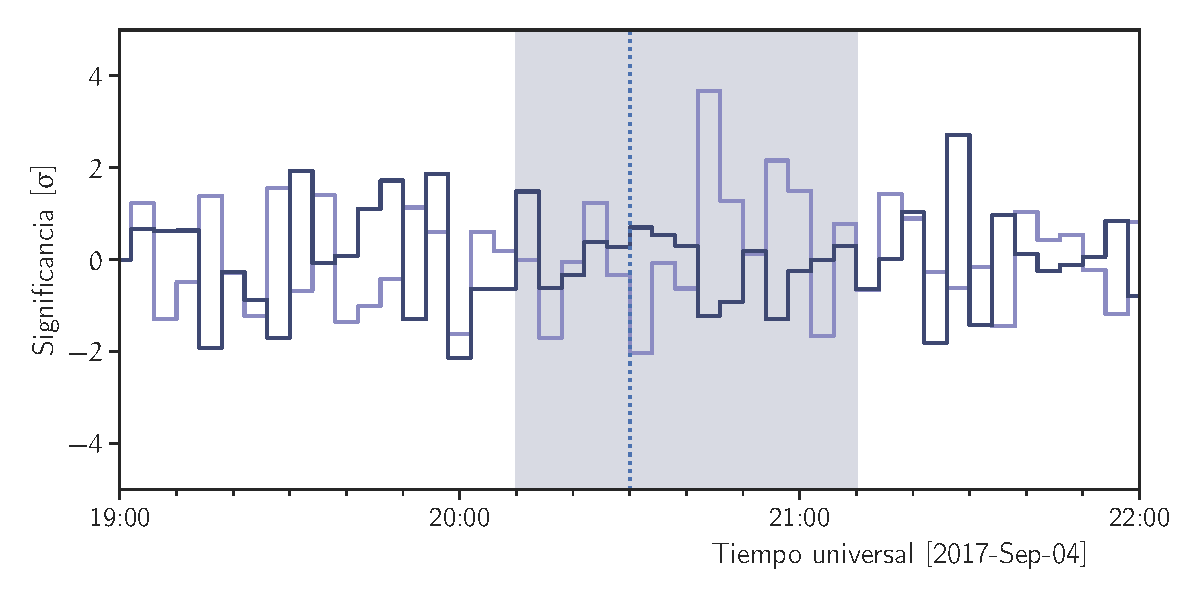
\includegraphics[width=\textwidth]{significance-170904.pdf}
\end{figure}

\end{frame}

\begin{frame}{Posible observación de neutrones el 04/09/17}

\begin{figure}
        \begin{subfigure}[b]{0.49\textwidth}
                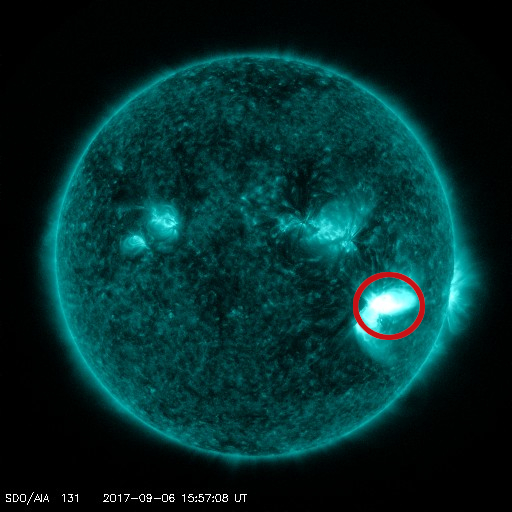
\includegraphics[width=6.85cm]{sdo170906-1550-13.jpg}
        \end{subfigure}
        \begin{subfigure}[b]{0.49\textwidth}
                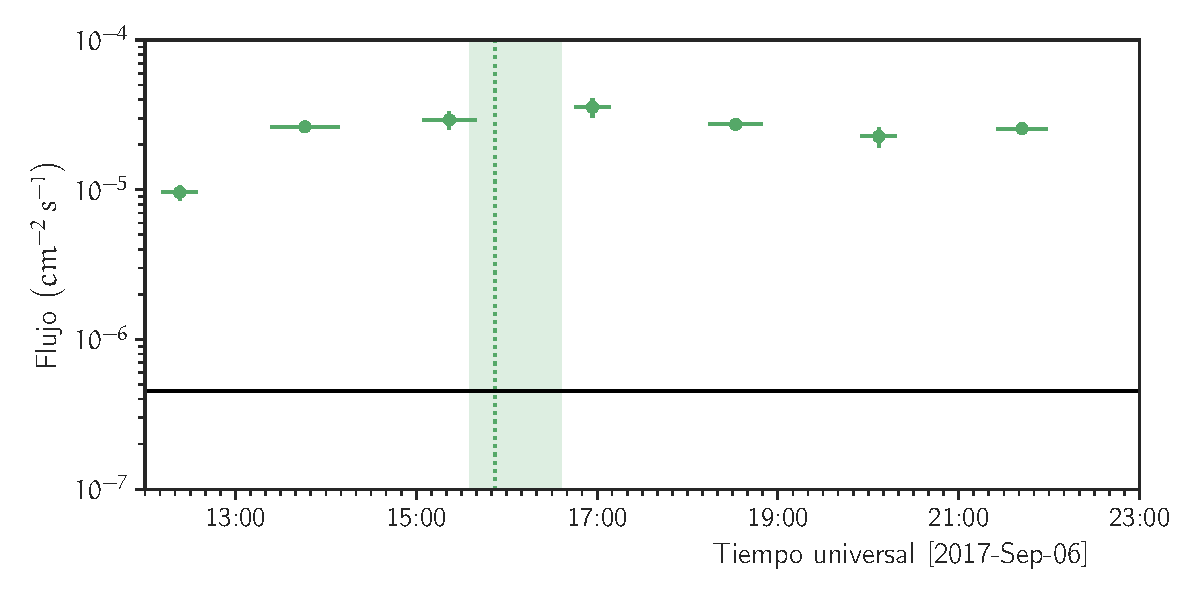
\includegraphics[width=6.85cm]{gammas-170906.pdf}
        \end{subfigure}
\end{figure}

\end{frame}

\begin{frame}{Resultados del análisis}

\begin{figure}
        \centering
        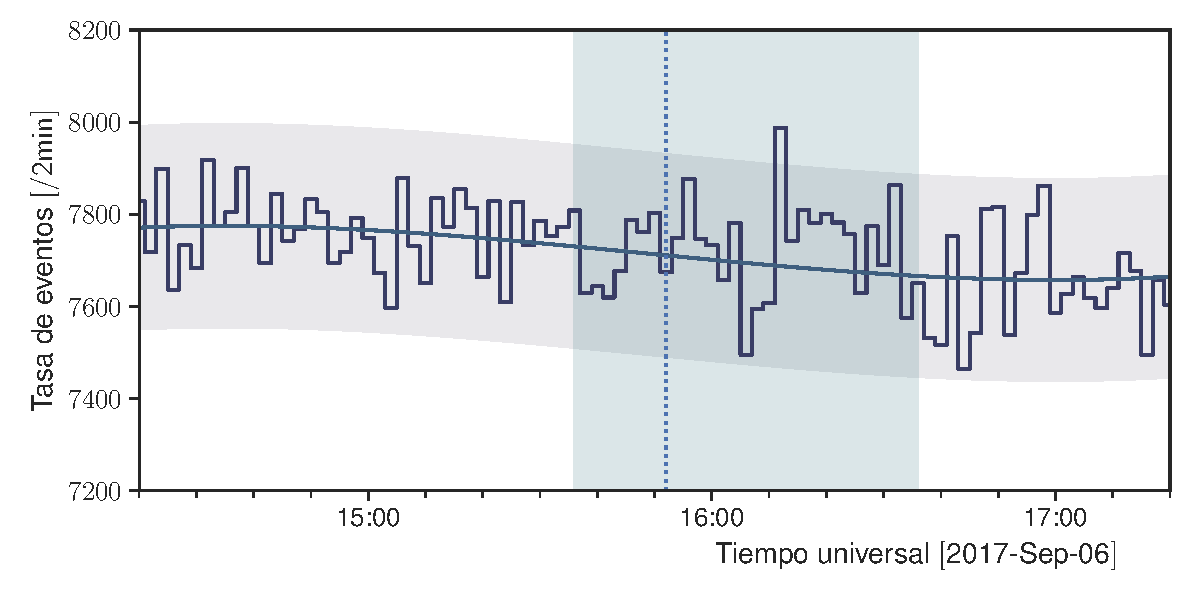
\includegraphics[width=\textwidth]{neutron-170906.pdf}
\end{figure}

\end{frame}


\begin{frame}{Resultados del análisis}

\begin{figure}
        \centering
        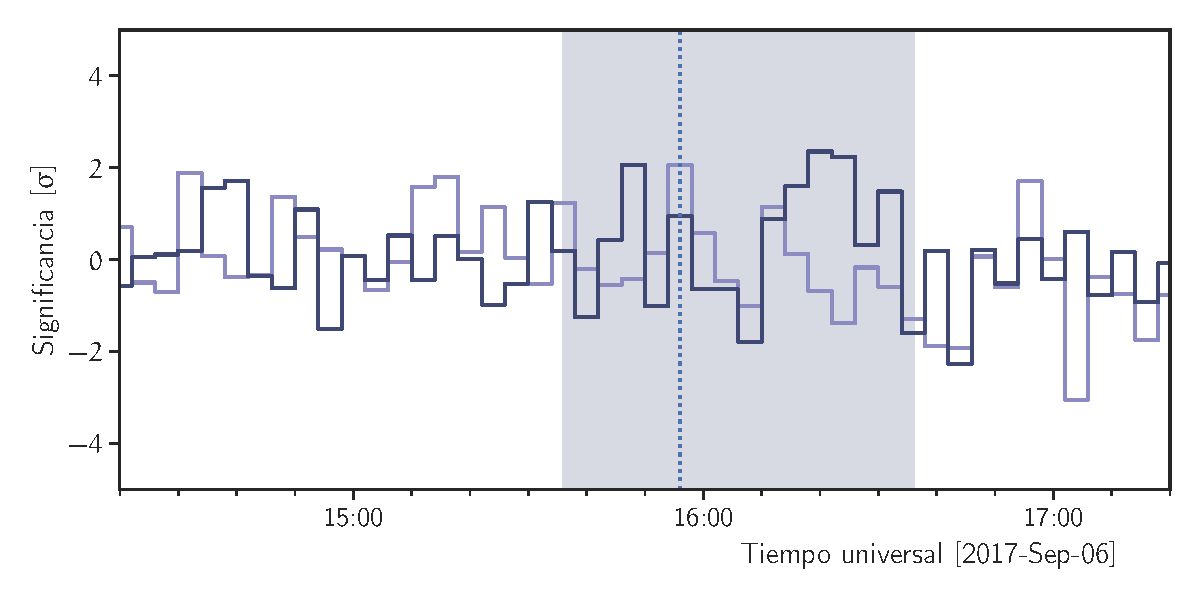
\includegraphics[width=\textwidth]{significance-170906.pdf}
\end{figure}

\end{frame}

\begin{frame}{Conclusiones}

\begin{block}{}

\begin{itemize}
	\item
\end{itemize}

\end{block}

\end{frame}


\end{document}
